\documentclass{article}
\usepackage[english,activeacute]{babel}
\usepackage[latin1]{inputenc}
\usepackage{amsmath,amsfonts,amssymb,amstext,amsthm,amscd}
\usepackage{graphicx}
\usepackage{here}
\usepackage{multicol}
\usepackage{listings}

\graphicspath{{images/}}
\lstset{
  language=VHDL,
  frame=single,
  breaklines=true,
  breakatwhitespace=true,
}
\usepackage{fancyhdr}
\setlength{\headheight}{15.2pt}
\usepackage[paperwidth=8.5in, paperheight=11.0in, top=1.0in, bottom=1.0in, left=1.0in, right=1.0in]{geometry}
\pagestyle{fancyplain}
\fancyhead[R]{LRT2022 Digital design}
\fancyhead[C]{}
\fancyhead[L]{Fall 2023}
\fancyfoot[L]{}
\fancyfoot[C]{\thepage}
\fancyfoot[R]{}

\begin{document}
\fancypagestyle{plain}{
	\renewcommand{\headrulewidth}{1pt}
	\renewcommand{\footrulewidth}{1pt}
}
\renewcommand{\footrulewidth}{1pt}
\renewcommand{\tablename}{Tabla}

\author{}
\title{Combinational logic circuits design}
\date{LIS}
\maketitle

\begin{abstract}
	The report delves into the design of two distinct combinational logic circuits: a water tank pump control system (watertank) and a coin detector mechanism (coin selector). The combinational circuits were formulated and analyzed based on the specified problem conditions and objectives. In the watertank circuit, the motor activation depended on the water levels in the cistern and tank, while the coin selector identified coins based on their heights. There is a truth table for both problems and a Karnaugh map for the watertank to obtain a boolean function. Both systems consider the errors as an event that should not activate anything in the outputs. The VHDL (VHSIC Hardware Description Language) programming methodologies used for the circuits varied; the watertank circuit employed concurrent signal assignments with logical operators, whereas the coin selector utilized conditional signal assignments. The circuits were simulated using EDA Playground and implemented on a Basys 3 board using Vivado 2018.2. The results were aligned with the expected outcomes, validating the designs.
	\textit{Keywords:}
\end{abstract}

\begin{multicols}{2}

	\subsection*{Objectives}\label{Objectives}

	\begin{enumerate}
		\item Design combinational logic circuits.
		\item Program and simulate custom combinational logic circuits in VHDL.
	\end{enumerate}

	\subsection*{Equipment}\label{Equipment}

	\begin{itemize}
		\item Basys 3 board
	\end{itemize}

	\subsection*{Software}\label{Software}

	\begin{itemize}
		\item Vivado 2018.2
		\item EDA Playground
	\end{itemize}

	\section*{Introduction and Theory}\label{Introduction}
	The following two circuits represent combinational circuits because based on the inputs, an output will be decided without depending on an specific logic gate design. One of the systems is designed with logic gates but that is only to match the table, therefore, it is still a combinational design since is the circuit the one matching the selections.

	Combinational circuits are digital circuits that produce an output based solely on the input. They are composed of logic gates that perform Boolean operations on the input signals. The output of a combinational circuit is determined by the current input values, and it does not depend on any previous input or output values. The basic combinational circuits include multiplexers, demultiplexers, decoders, encoders, and comparators \cite{floyd_digital_2023}.

	A Karnaugh map is a visual representation of a truth table. It is a two-dimensional grid where each cell represents a possible combination of input values. The cells are arranged so that adjacent cells differ by only one input value. The truth table and the Karnaugh map are equivalent representations of the same Boolean function. The truth table lists all possible input combinations and their corresponding output values, while the Karnaugh map shows how the input combinations can be grouped to simplify the Boolean expression \cite{allaboutcircuits}.

	Through the use of the Karnaugh map I was able to represent a combinational circuit with logic gates. With this, I was able to fulfill the goal of this laboratory which is to demonstrate the use case of combinational circuits found in daily situations. The two circuits presented here are one of a pump control system which will be called watertank and one of a coin detector which will be called coin selector for simplicity purposes.

	\begin{figure}[H]
		\centering
		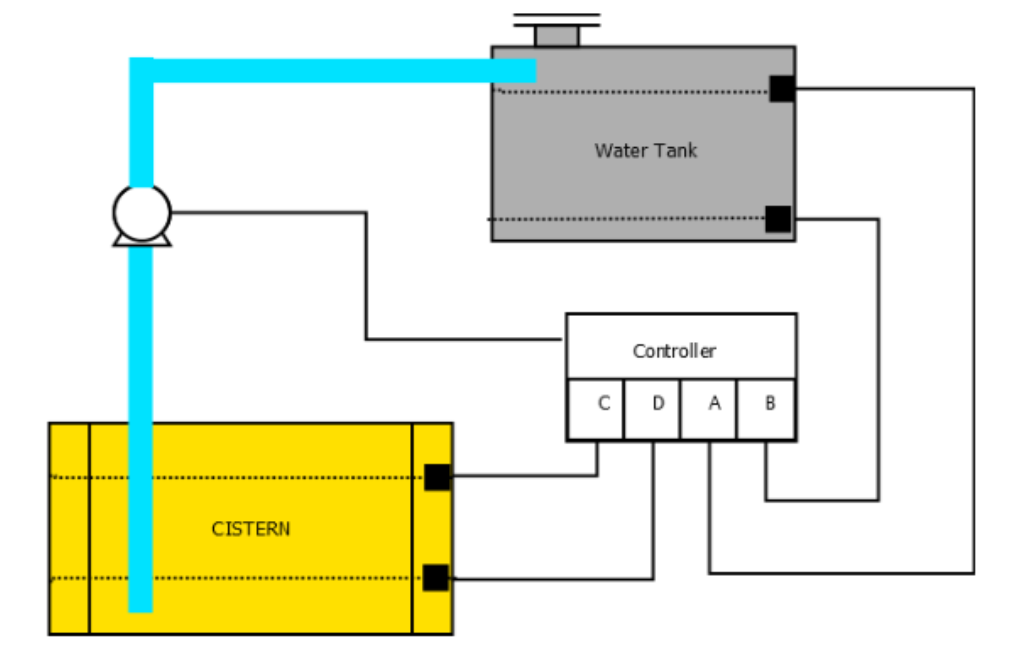
\includegraphics[width=0.8\linewidth]{images/diagrams/watertank/pump.png}
		\caption{Pump control \cite{Torres}}
		\label{Pump control Diagram}
	\end{figure}

	\begin{figure}[H]
		\centering
		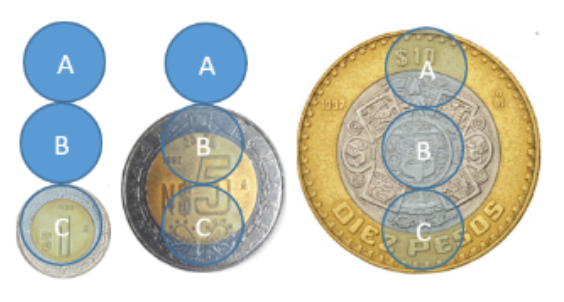
\includegraphics[width=0.8\linewidth]{images/diagrams/coin-selector/coin-detector.png}
		\caption{Coin detector \cite{Torres}}
		\label{Coin detector Diagram}
	\end{figure}

	For the following analysis and results, the testbench in VHDL code and the images of the Basys 3 results will not be complete and will be anexed at the end of the report. The reason for this is that the testbench and the images are too long to be included in the report and it will be easier to read if they are in the appendix.

	\section*{Analysis}\label{Analysis}
	This is the thoerical analysis of both problems of the watertank and the coin selector.

	\subsection*{Watertank}\label{Watertank Analysis}
	The watertank consists of pumping water to the system when necessary. The problem conditions are that water can only be pumped (Activate M which is the motor with signal 1) when the cistern is not empty and the tank is not full. The cistern is the one that provides the water to the system and the tank is the one that stores the water. Signal 1 corresponds to active state and signal 0 corresponds to unactive state. A, B, C, D are active when water is present. As extra conditions, when only the high levels of the cistern or the watertank are active, the pump should not activate because it might be an error since the bottom part is not detecting any water.

	\subsubsection*{Boolean tables}\label{Watertank Boolean tables}
	Considering the previous description of the problem and the conditions of the design that will be implemented, the following truth table was created. A corresponds to the tank high state; B corresponds to the tank low state; C corresponds to the cistern high state; D corresponds to the cistern low state; M corresponds to the motor state.

	\begin{table}[H]
		\centering
		\caption{Watertank truth table}
		\vspace*{1em}
		\begin{tabular}{|l|l|l|l|l|}
			\hline
			A & B & C & D & M \\ \hline
			0 & 0 & 0 & 0 & 0 \\ \hline
			0 & 0 & 0 & 1 & 1 \\ \hline
			0 & 0 & 1 & 0 & 0 \\ \hline
			0 & 0 & 1 & 1 & 1 \\ \hline
			0 & 1 & 0 & 0 & 0 \\ \hline
			0 & 1 & 0 & 1 & 1 \\ \hline
			0 & 1 & 1 & 0 & 0 \\ \hline
			0 & 1 & 1 & 1 & 1 \\ \hline
			1 & 0 & 0 & 0 & 0 \\ \hline
			1 & 0 & 0 & 1 & 0 \\ \hline
			1 & 0 & 1 & 0 & 0 \\ \hline
			1 & 0 & 1 & 1 & 0 \\ \hline
			1 & 1 & 0 & 0 & 0 \\ \hline
			1 & 1 & 0 & 1 & 0 \\ \hline
			1 & 1 & 1 & 0 & 0 \\ \hline
			1 & 1 & 1 & 1 & 0 \\ \hline
		\end{tabular}
	\end{table}

	\subsubsection*{Karnaugh map}\label{Watertank Karnaugh map}

	The Karnaugh map of 4 variables is the following. We can form a group with 4 ones. When solving for it, we notice that when A is not active and D is active the active states appear. With that information we can create the boolean function that represents the truth table of this combinational circuit M(A, B, C, D) = A'D.

	\begin{figure}[H]
		\centering
		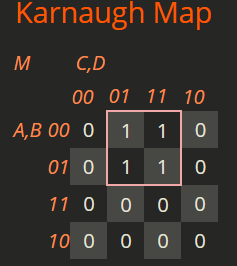
\includegraphics[width=0.8\linewidth]{images/k-maps/watertank.png}
		\caption{Watertank Karnaugh map}
		\label{Watertank Karnaugh map solution}
	\end{figure}

	\subsubsection*{VHDL}\label{Watertank VHDL}

	With the boolean function M(A, B, C, D) = A'D we can create the following VHDL code by using the concurrent signal assignments with logical operators method.

	\lstinputlisting[caption=Watertank VHDL code]{codes/motor-control.vhd}

	To test the code, the following testbench was created.

	\lstinputlisting[caption=Watertank testbench,firstline=1,lastline=15]{codes/motor-control-tests.vhd}

	Using EDA Playground, the following simulation was obtained as an EPWave. We can notice that the motor is only active when the cistern is not empty and the tank is not full. Also when only the high levels of the cistern or the watertank are active, the pump is not activated. So we can conclude that the design implementation is correct.

	\begin{figure}[H]
		\centering
		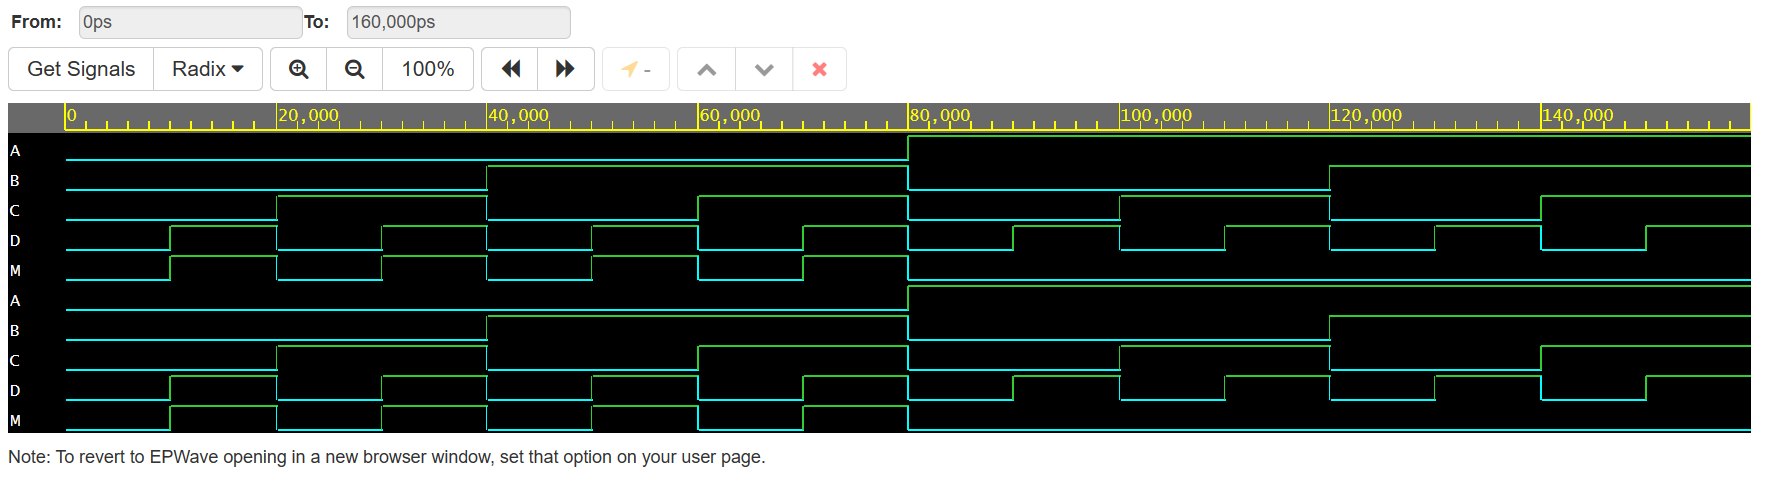
\includegraphics[width=1\linewidth]{images/waves/watertank.png}
		\caption{Watertank simulation}
		\label{Watertank simulation}
	\end{figure}

	\subsection*{Coin selector}\label{Coin selector Analysis}

	There are 3 heights in the coins. When height C is active, the coin of value 1 is active. When C and B are active, the coin of value 5 is active. When A, B and C are active, the coin of value 10 is active. We can also make the similar conditions as the previous combinational circuit where when only the high levels of the coin selector are active, the coin selector should not activate because it might be an error since the bottom part is not detecting any coin. We can also suppose that the B should not be activated alone. So A nor B should be activated alone when C is not active. We will call the value of 10 as Diez, the value of 5 as Cinco and the value of 1 as Uno. A, B, C are active when a part of a coin is present. Diez, Cinco, Uno are active when the coin of that value is present.

	\subsubsection*{Boolean tables}\label{Coin selector Boolean tables}

	So at the end we have only 3 possible states represented in the following truth table.

	\begin{table}[H]
		\centering
		\caption{Coin selector truth table}
		\vspace*{1em}
		\begin{tabular}{|l|l|l|l|l|l|}
			\hline
			A & B & C & Diez & Cinco & Uno \\ \hline
			0 & 0 & 0 & 0    & 0     & 0   \\ \hline
			0 & 0 & 1 & 0    & 0     & 1   \\ \hline
			0 & 1 & 0 & 0    & 0     & 0   \\ \hline
			0 & 1 & 1 & 0    & 1     & 0   \\ \hline
			1 & 0 & 0 & 0    & 0     & 0   \\ \hline
			1 & 0 & 1 & 0    & 0     & 0   \\ \hline
			1 & 1 & 0 & 0    & 0     & 0   \\ \hline
			1 & 1 & 1 & 1    & 0     & 0   \\ \hline
		\end{tabular}
		\label{Coin selector truth table}
	\end{table}

	\subsubsection*{Karnaugh map}\label{Coin selector Karnaugh map}

	For this one, since there are only 3 states which are simple we can skip the Karnaugh map and use a different type of code design.

	\subsubsection*{VHDL}\label{Coin selector VHDL}
	For this code, the conditional signal assignments was chosen for the simplicity of the table cases. When the cases that meet a coin be active are meeted, the code will return the active state for a coin, else it will return the unactive state for a coin.

	\lstinputlisting[caption=Coin selector VHDL code]{codes/coin-selector.vhd}

	To test the code, the following testbench was created.

	\lstinputlisting[caption=Coin selector testbench,firstline=1,lastline=15]{codes/coin-selector-test.vhd}

	Using EDA Playground, the following simulation was obtained as an EPWave. The corresponding coin is active when the proper detectors are active. So we can conclude that the design implementation is correct.

	\begin{figure}[H]
		\centering
		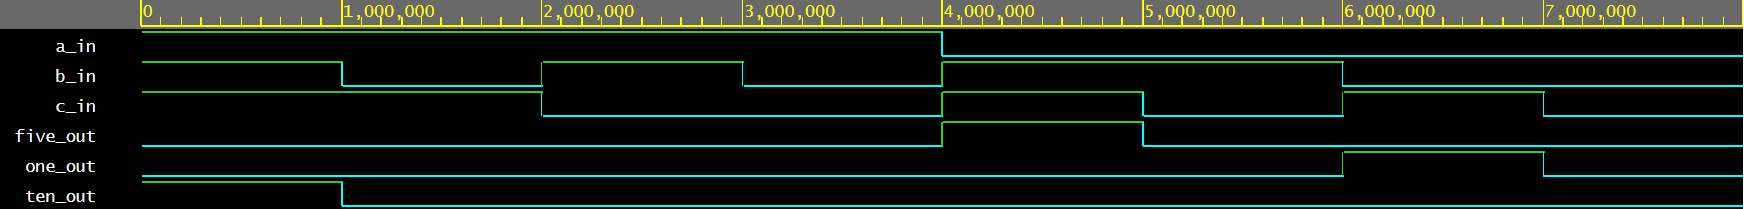
\includegraphics[width=1\linewidth]{images/waves/coin-selector.png}
		\caption{Coin selector simulation}
		\label{Coin selector simulation}
	\end{figure}

	\section*{Records}\label{Records}
	The second part of this report is to demonstrate this in a real board. For this, the Basys 3 board was used. The following images show the implementation of the watertank and the coin selector in the board.

	\subsection*{Watertank}\label{Watertank Records}

	To show that the circuit is properly working, we will compare to the states shown in the tables. A consideration is that SW0 corresponds to A, SW1 corresponds to B, SW2 corresponds to C, and SW3 corresponds to D. The LED0 corresponds to M. These leds and switches are numbered from right to left. For both tables, we consider the first element after the headers as element 0, then the second element as element 1 and so on. For the watertank, we will consider the element 2 which has floating water and should not turn on, the element 13 where the water tank is full and has water in the cistern and should not turn on, and the element 3 which has full cistern and no water in the watertank so it should turn on.

	Here the C is on, the others are off, the water is floating so the tank should be off.

	\begin{figure}[H]
		\centering
		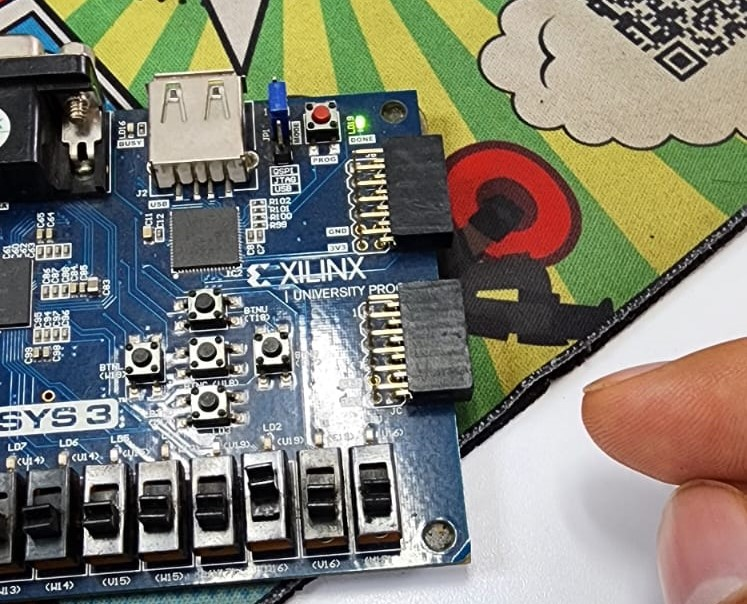
\includegraphics[width=0.8\linewidth]{images/diagrams/watertank/watertank2.jpg}
		\caption{Watertank element 2}
		\label{Watertank element 2}
	\end{figure}

	Here the A, B, D are on, C is off so the tank is high and should be off.

	\begin{figure}[H]
		\centering
		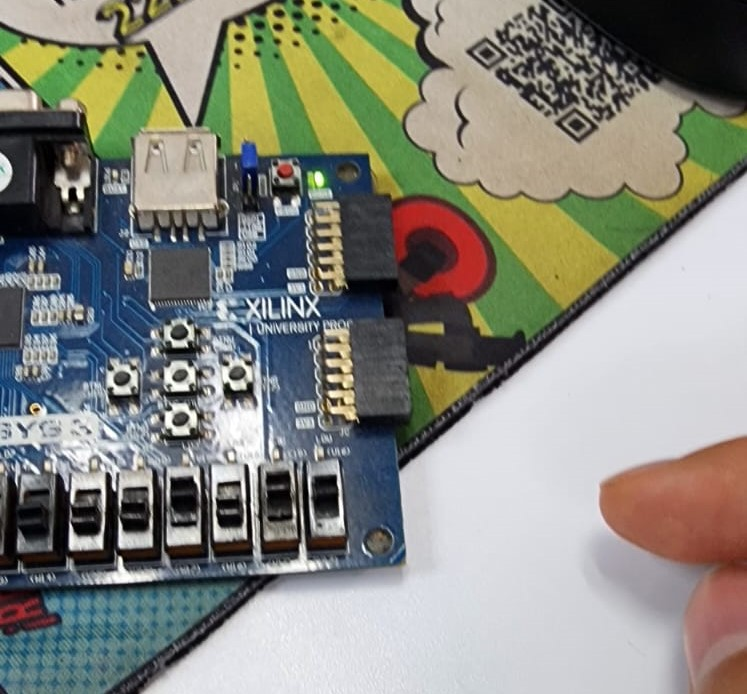
\includegraphics[width=0.8\linewidth]{images/diagrams/watertank/watertank13.jpg}
		\caption{Watertank element 13}
		\label{Watertank element 13}
	\end{figure}

	For element 3, it has C and D on, full cistern and no water in the water tank, A and B are off so the pump (M) turns on.

	\begin{figure}[H]
		\centering
		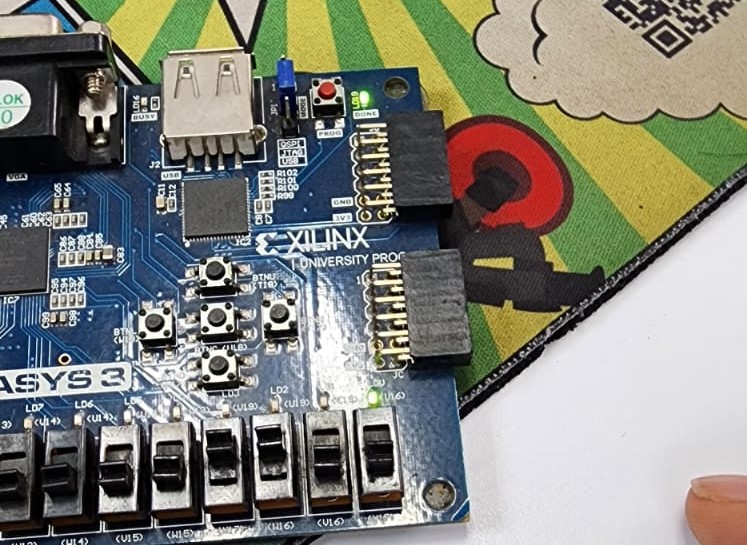
\includegraphics[width=0.8\linewidth]{images/diagrams/watertank/watertank3.jpg}
		\caption{Watertank element 3}
		\label{Watertank element 3}
	\end{figure}

	\subsection*{Coin selector}\label{Coin selector Records}

	To show that the circuit is properly working, we will compare to the states shown in the tables. A consideration is that SW0 corresponds to A, SW1 corresponds to B, SW2 corresponds to C. LD0 corresponds to Diez, LD1 corresponds to Cinco, LD2 corresponds to Uno. These leds and switches are numbered from right to left. For both tables, we consider the first element after the headers as element 0, then the second element as element 1 and so on. For the coin selector, we will consider the element 0 which has no coin and should not turn on, the element 1 where the coin of value 1 is present and should turn on, the element 7 which has the coin of value 10 and should turn on, and the element 3 which has the coin of value 5 and should turn on. As example of floating values the element 4 has A turned on and the others off, so no coin should be detected.

	Here the A, B, C are off, so no coin should be detected.

	\begin{figure}[H]
		\centering
		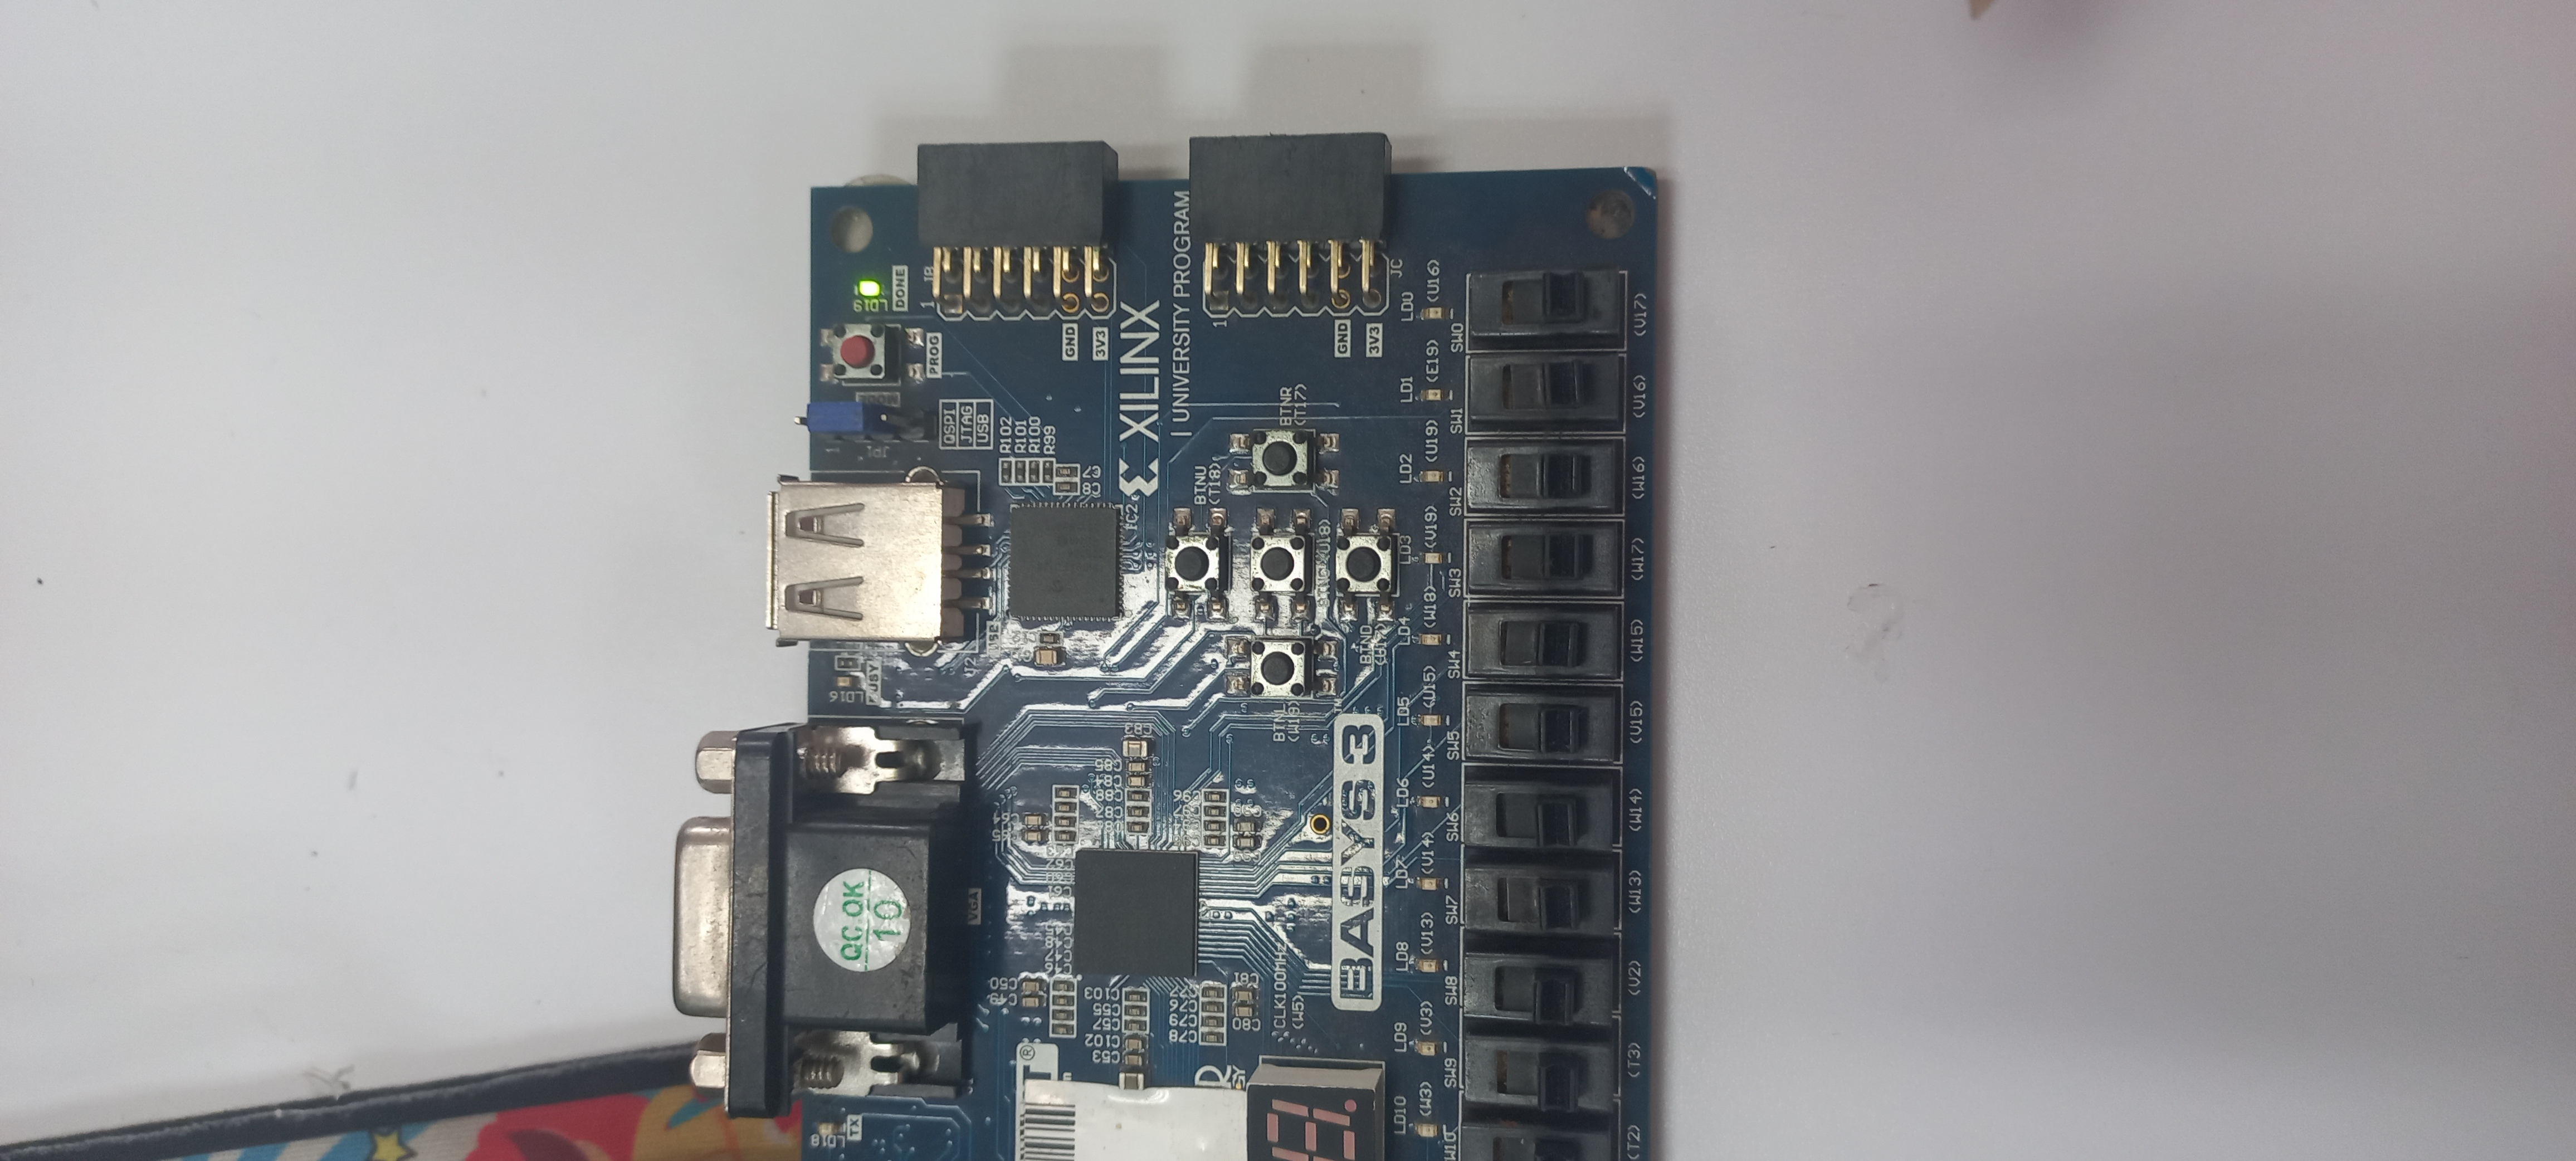
\includegraphics[width=0.8\linewidth]{images/diagrams/coin-selector/coin-selector0.jpg}
		\caption{Coin selector element 0}
		\label{Coin selector element 0}
	\end{figure}

	Here the C is on, the others are off, so the coin of value 1 should be detected.

	\begin{figure}[H]
		\centering
		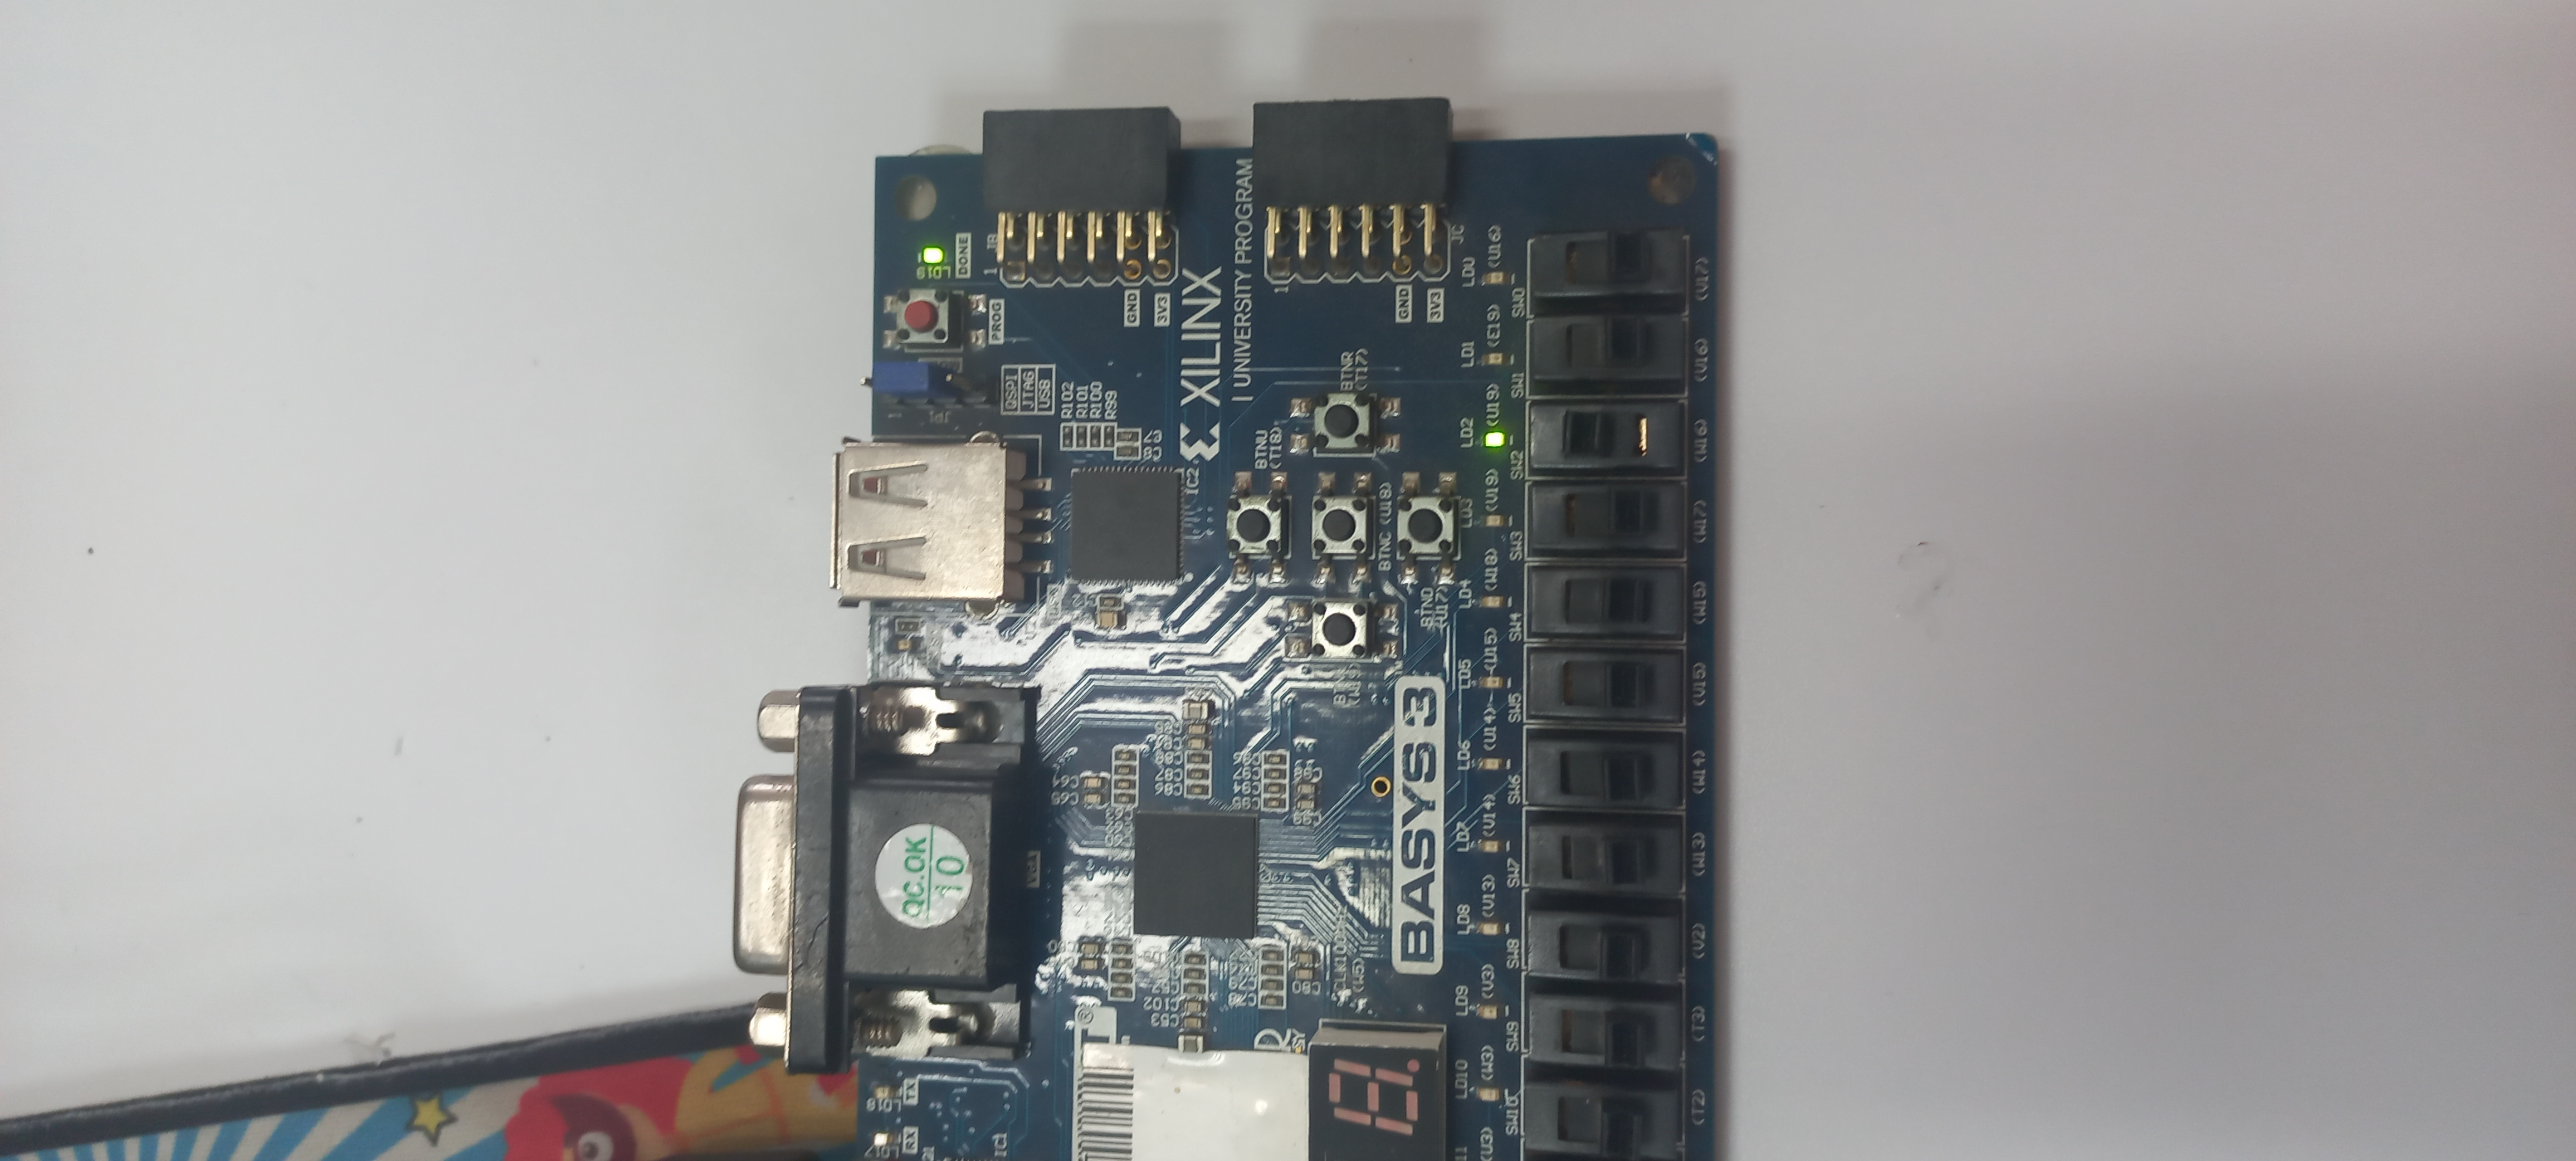
\includegraphics[width=0.8\linewidth]{images/diagrams/coin-selector/coin-selector1.jpg}
		\caption{Coin selector element 1}
		\label{Coin selector element 1}
	\end{figure}

	Here the A, B, C are on, so the coin of value 10 should be detected.

	\begin{figure}[H]
		\centering
		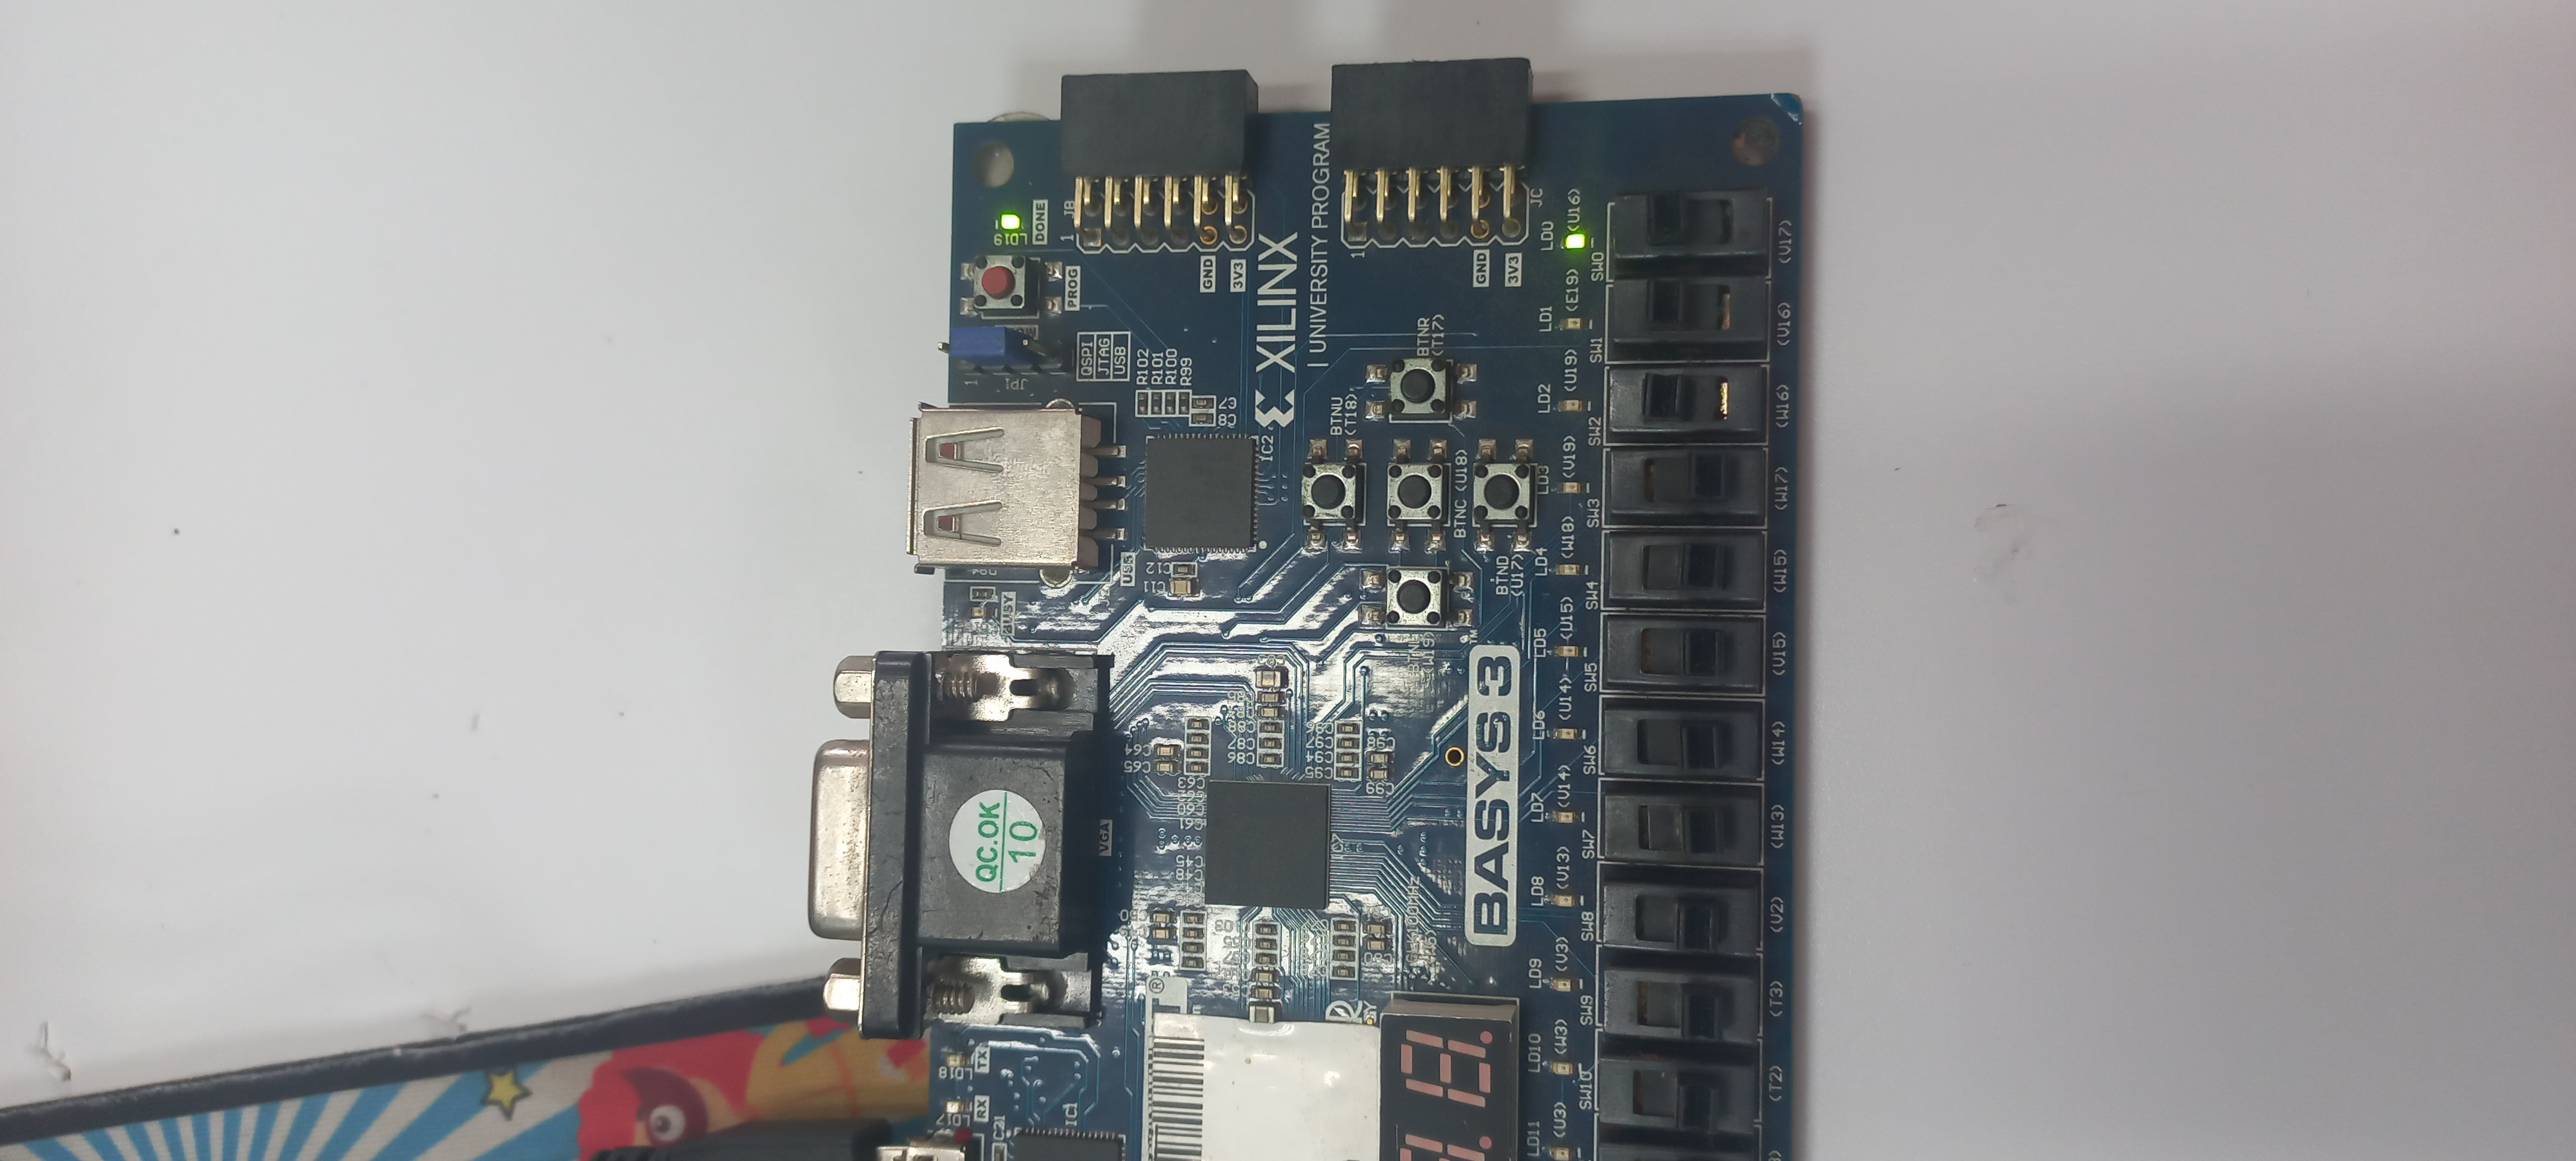
\includegraphics[width=0.8\linewidth]{images/diagrams/coin-selector/coin-selector7.jpg}
		\caption{Coin selector element 7}
		\label{Coin selector element 7}
	\end{figure}

	Here the B, C are on, the others are off, so the coin of value 5 should be detected.

	\begin{figure}[H]
		\centering
		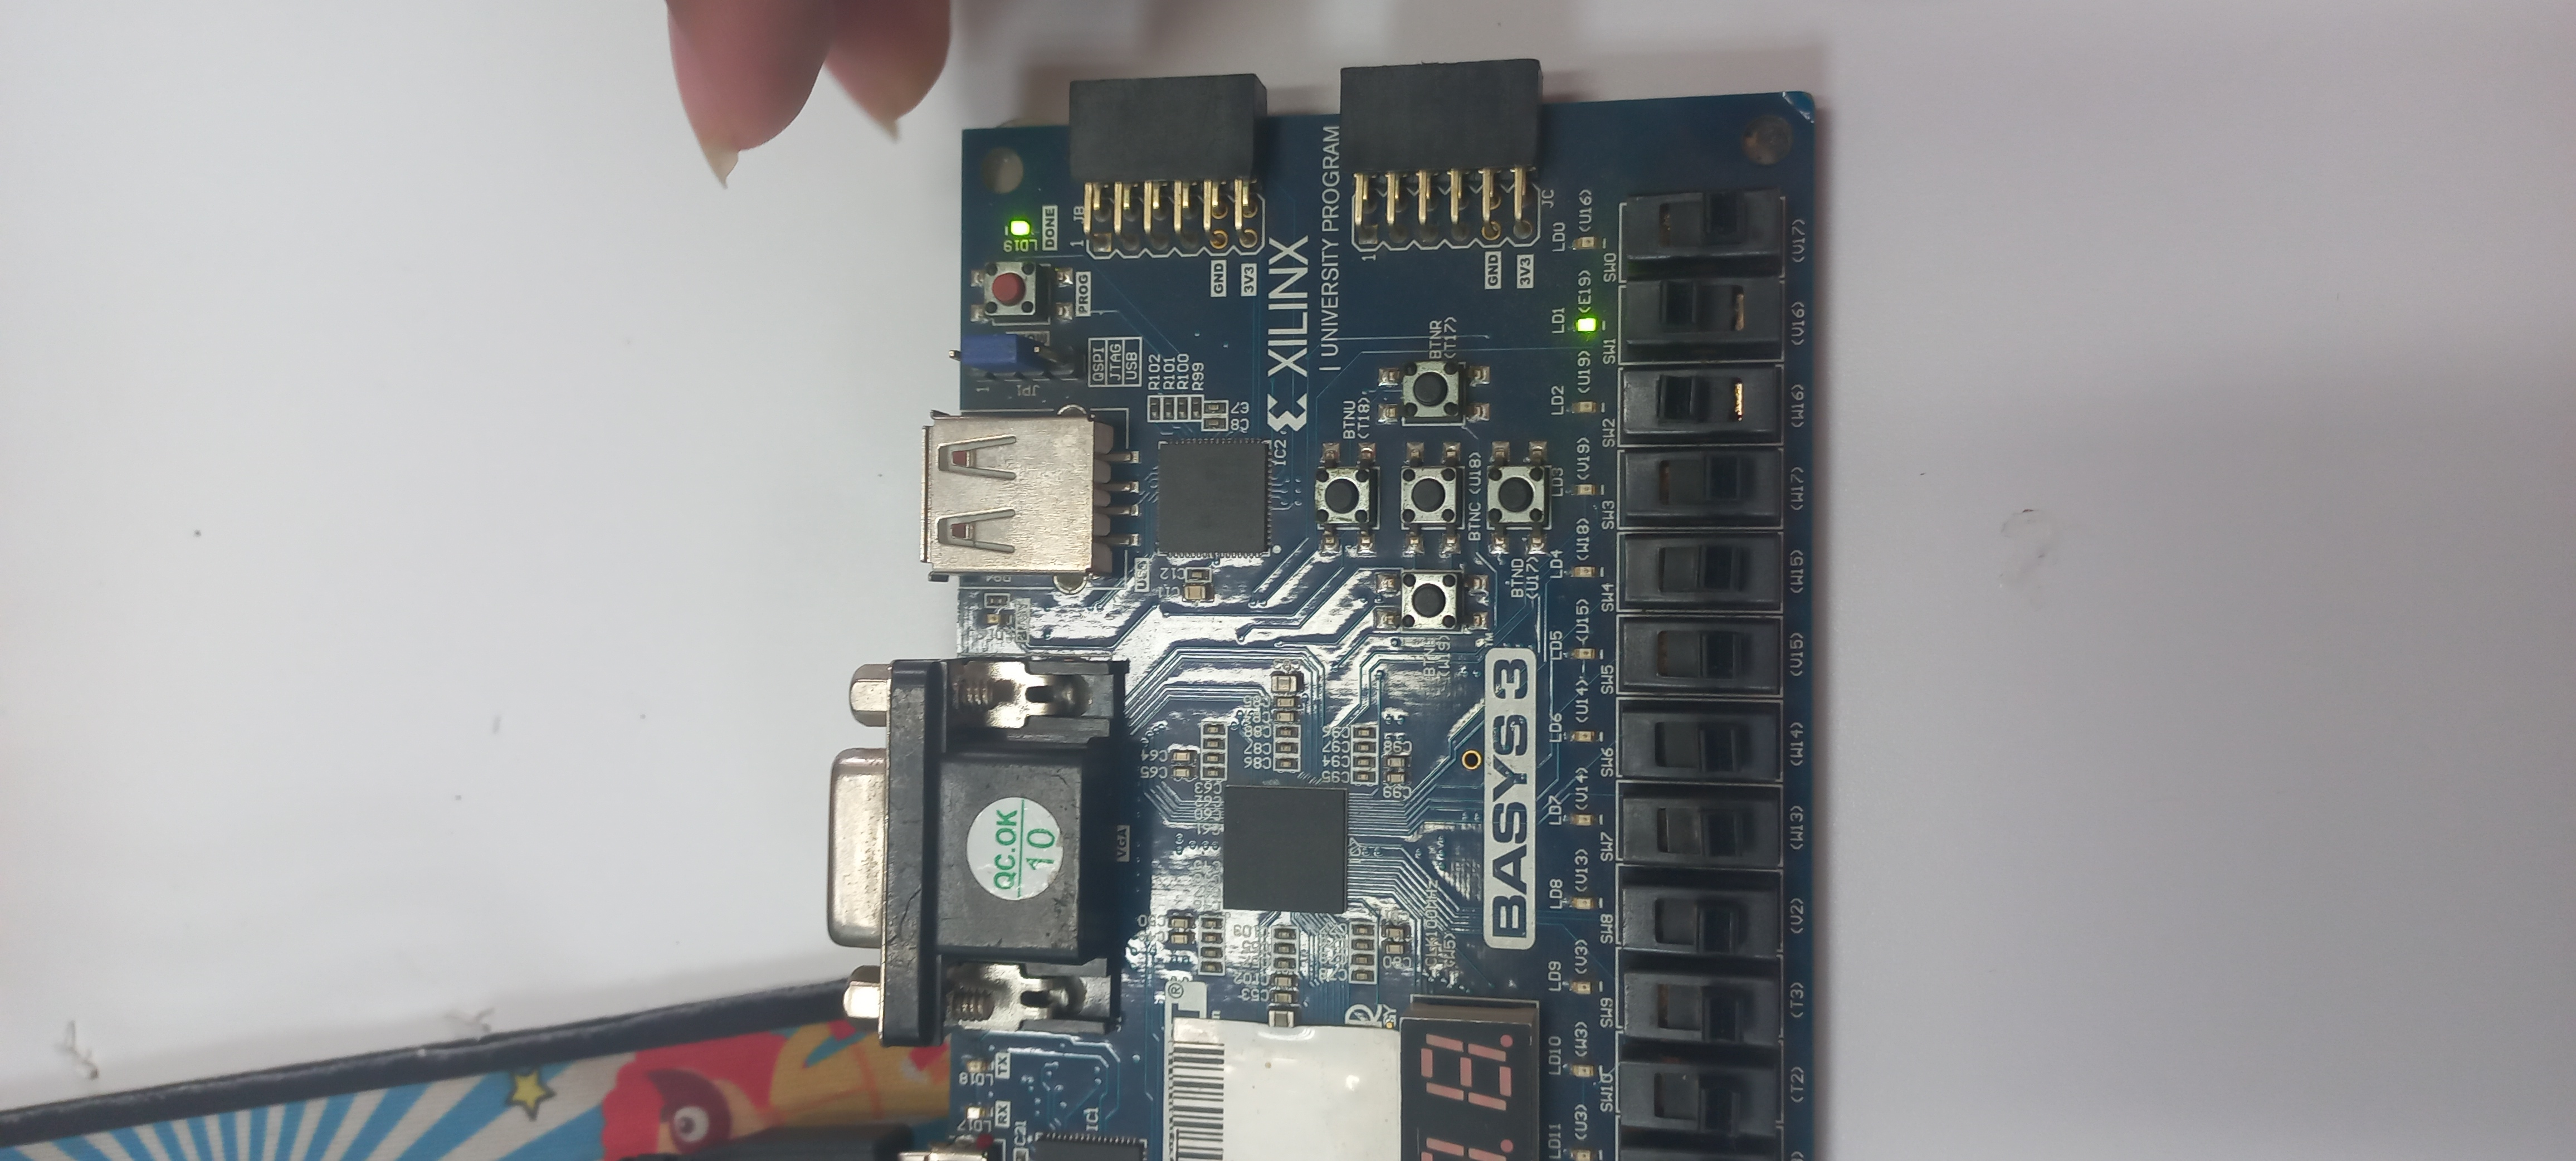
\includegraphics[width=0.8\linewidth]{images/diagrams/coin-selector/coin-selector3.jpg}
		\caption{Coin selector element 3}
		\label{Coin selector element 3}
	\end{figure}

	Here A is on, the others are off, so no coin should be detected.

	\begin{figure}[H]
		\centering
		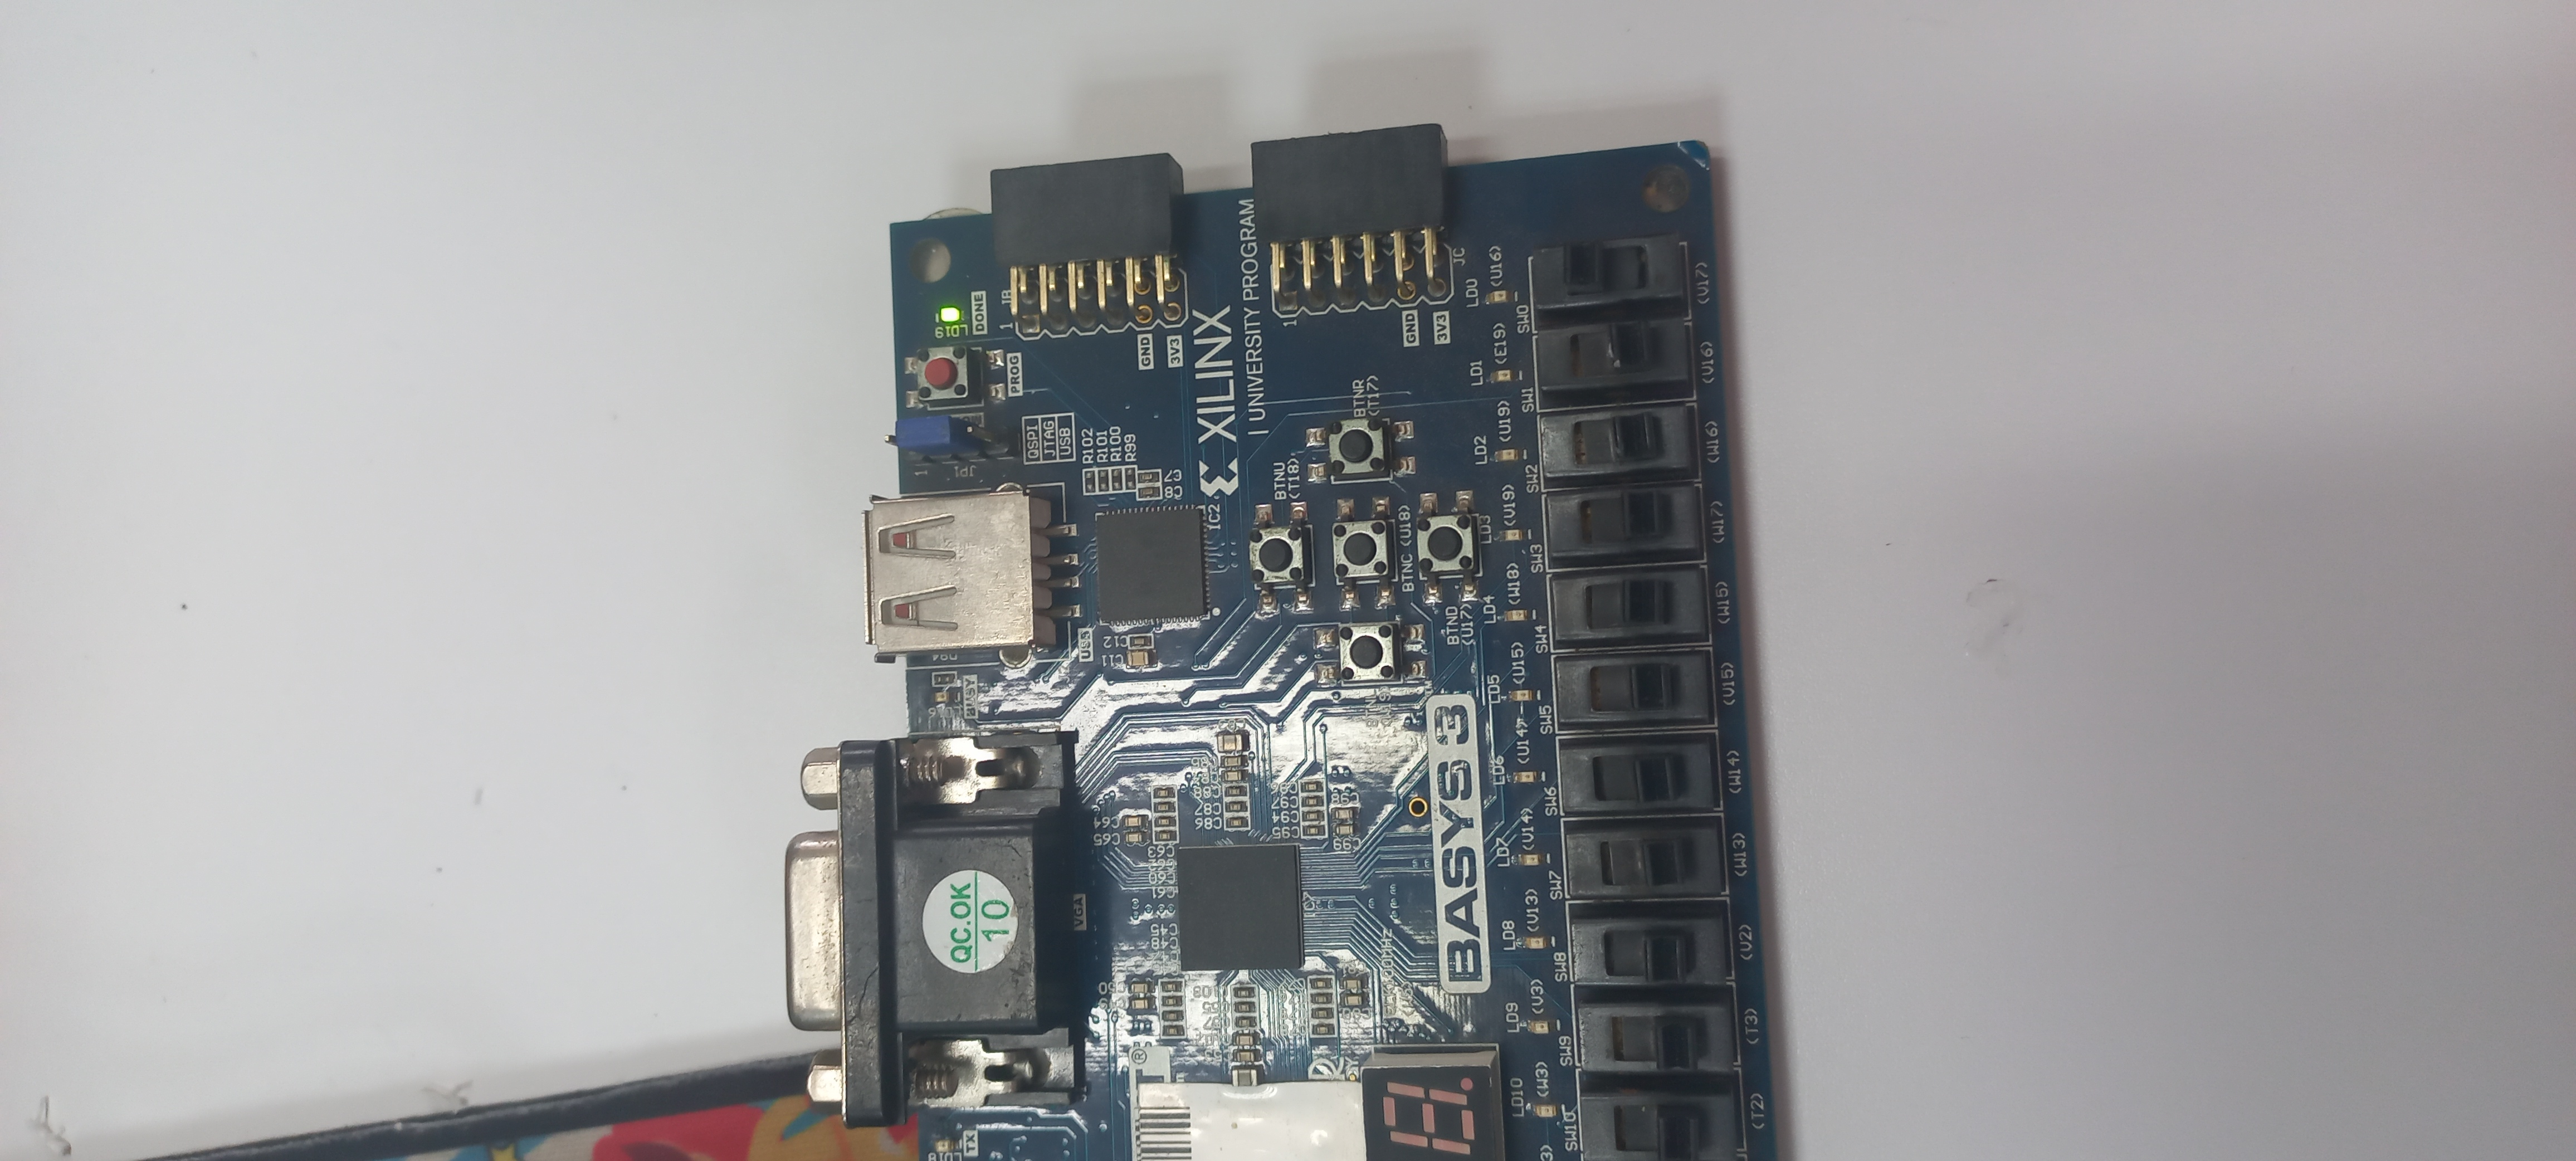
\includegraphics[width=0.8\linewidth]{images/diagrams/coin-selector/coin-selector4.jpg}
		\caption{Coin selector element 4}
		\label{Coin selector element 4}
	\end{figure}

	\section*{Conclusions}\label{Conclusions}
	The exploration into the design of the watertank and coin selector combinational circuits demonstrated how these circuits can efficiently represent and solve real-world problems. The watertank circuit was crafted to ensure that water is pumped only under specific conditions, and the results aptly confirmed the design's accuracy. On the other hand, the coin selector circuit was adept at distinguishing between coins of varying sizes. The selection of different VHDL programming methodologies for the circuits showcased how diverse coding styles can be employed based on the problem's requirements and the designer's preferences. The successful simulations and implementations affirmed the practical applicability of these combinational circuits in electronic systems.

	Additionally, while the concept of 'don't cares' in logic design could have been utilized to simplify the circuit designs, it was not incorporated in this study. 'Don't cares' can be advantageous when the designer wants to allow flexibility for certain input conditions, possibly optimizing and minimizing the circuit's complexity. However, in this case, all conditions and inputs needed to be explicitly defined and addressed, ensuring that the circuits behaved predictably for all scenarios. This approach guarantees the precision and reliability of the circuits, as each input directly correlates to a specific output or action. This study underscores the significance of careful design, simulation, and consideration of all potential inputs in creating reliable and functional digital solutions.

	\newpage
	\appendix

	\section{Codes}\label{Codes}

	\lstinputlisting[caption=Watertank VHDL code]{codes/motor-control.vhd}

	\lstinputlisting[caption=Watertank testbench]{codes/motor-control-tests.vhd}

	\lstinputlisting[caption=Coin selector VHDL code]{codes/coin-selector.vhd}

	\lstinputlisting[caption=Coin selector testbench]{codes/coin-selector-test.vhd}

	\section{Images}\label{Images}

	\begin{figure}[H]
		\centering
		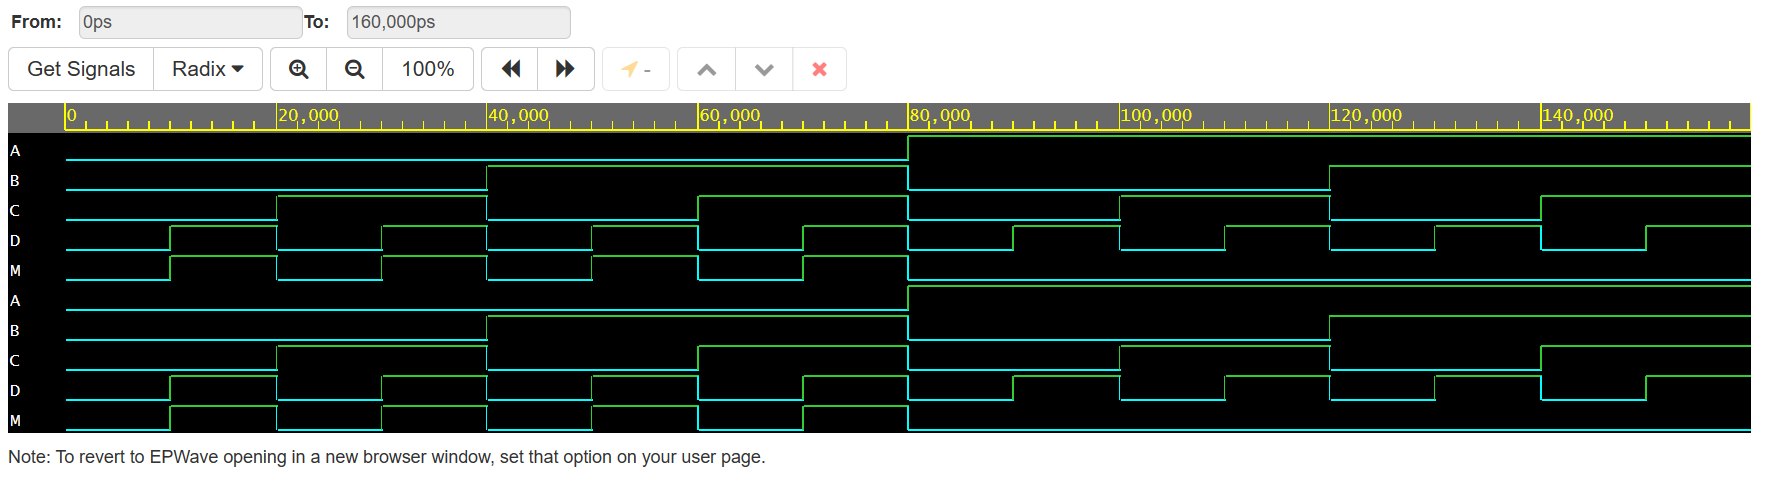
\includegraphics[width=0.8\linewidth]{images/waves/watertank.png}
		\caption{Watertank simulation}
		\label{Watertank simulation Apendix}
	\end{figure}

	\begin{figure}[H]
		\centering
		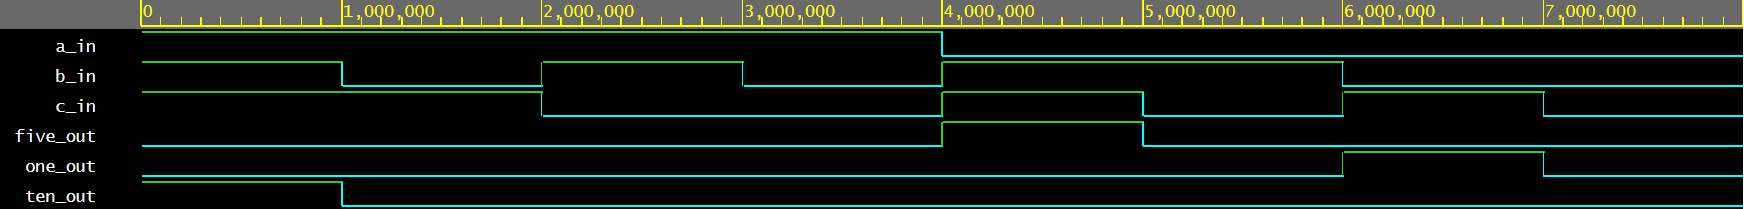
\includegraphics[width=0.8\linewidth]{images/waves/coin-selector.png}
		\caption{Coin selector simulation}
		\label{Coin selector simulation Apendix}
	\end{figure}

	\begin{figure}[H]
		\centering
		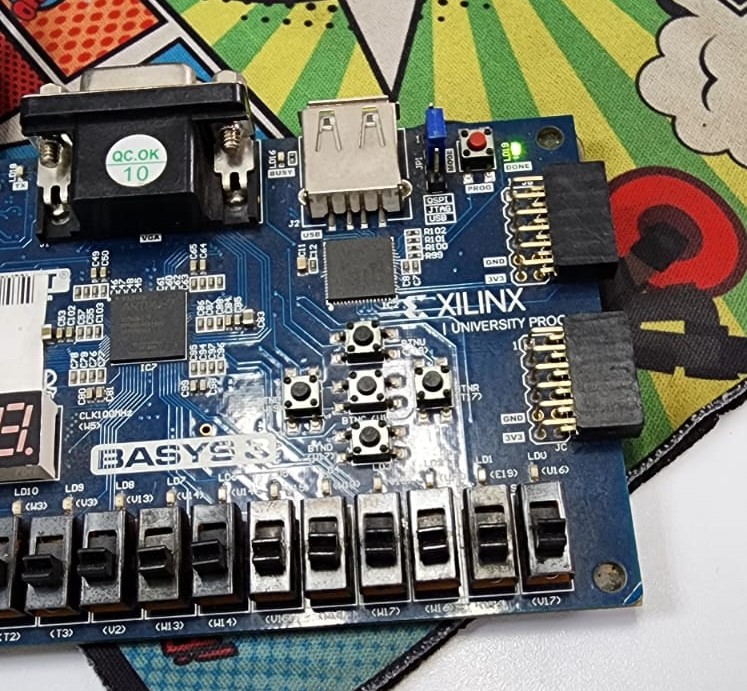
\includegraphics[width=0.8\linewidth]{images/diagrams/watertank/watertank0.jpg}
		\caption{Watertank element 0}
		\label{Watertank element 0 Apendix}
	\end{figure}

	\begin{figure}[H]
		\centering
		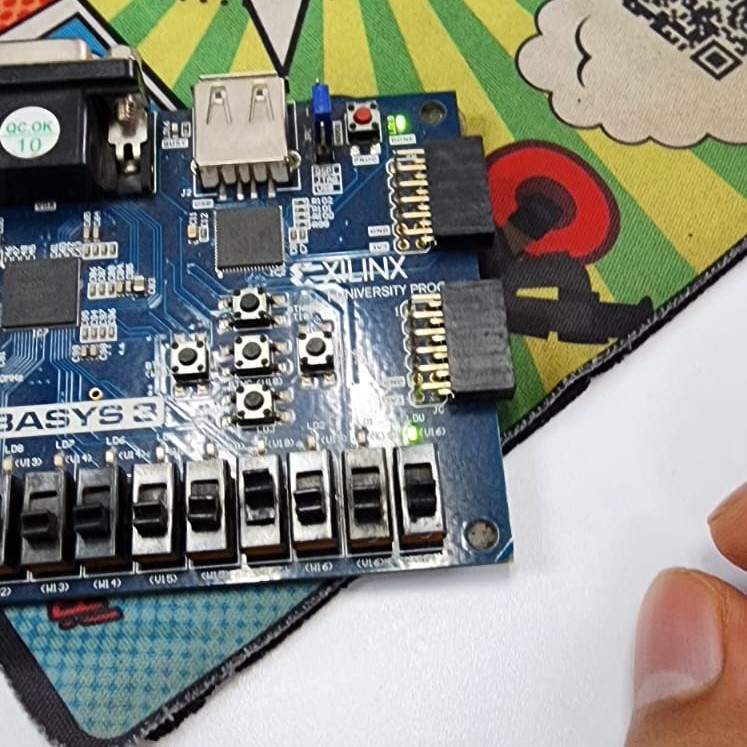
\includegraphics[width=0.8\linewidth]{images/diagrams/watertank/watertank1.jpg}
		\caption{Watertank element 1}
		\label{Watertank element 1 Apendix}
	\end{figure}

	\begin{figure}[H]
		\centering
		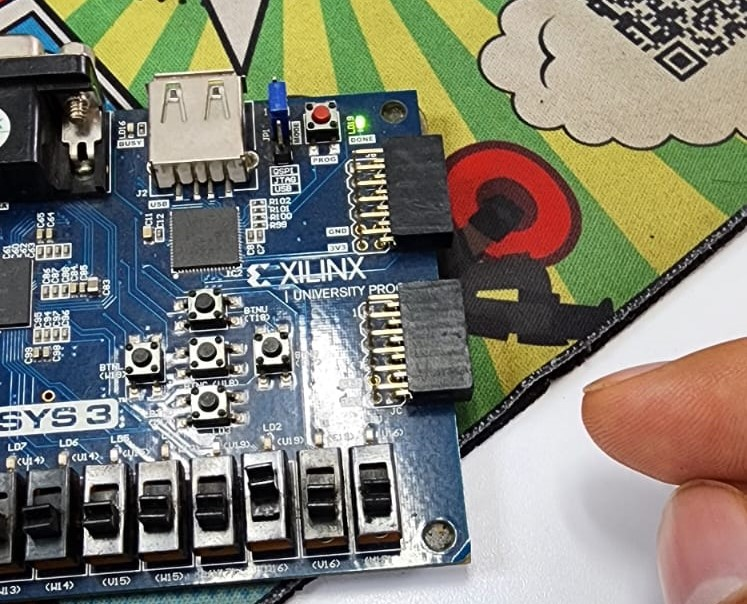
\includegraphics[width=0.8\linewidth]{images/diagrams/watertank/watertank2.jpg}
		\caption{Watertank element 2}
		\label{Watertank element 2 Apendix}
	\end{figure}

	\begin{figure}[H]
		\centering
		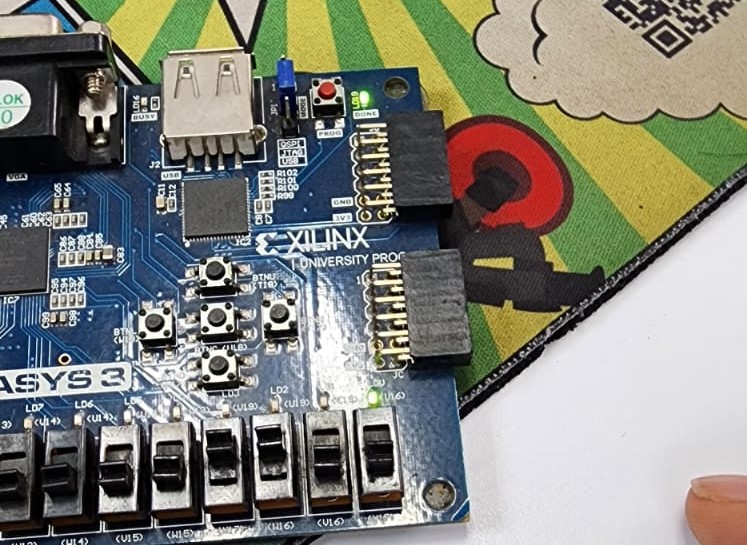
\includegraphics[width=0.8\linewidth]{images/diagrams/watertank/watertank3.jpg}
		\caption{Watertank element 3}
		\label{Watertank element 3 Apendix}
	\end{figure}

	\begin{figure}[H]
		\centering
		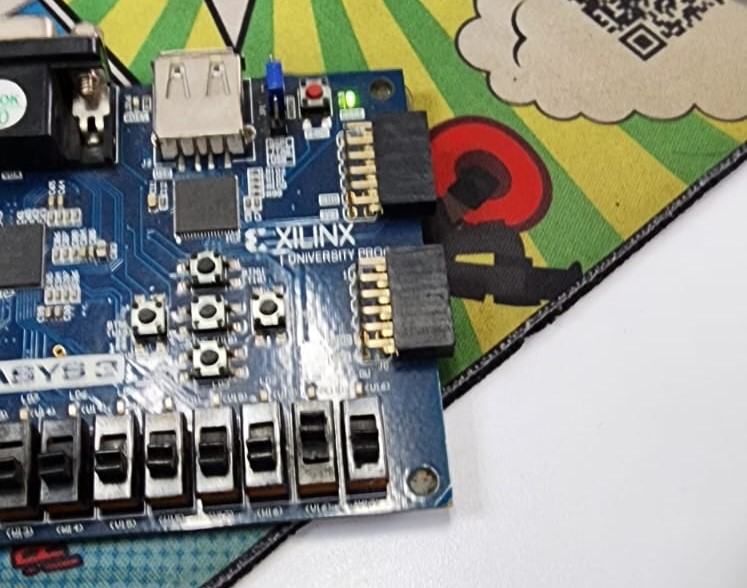
\includegraphics[width=0.8\linewidth]{images/diagrams/watertank/watertank4.jpg}
		\caption{Watertank element 4}
		\label{Watertank element 4 Apendix}
	\end{figure}

	\begin{figure}[H]
		\centering
		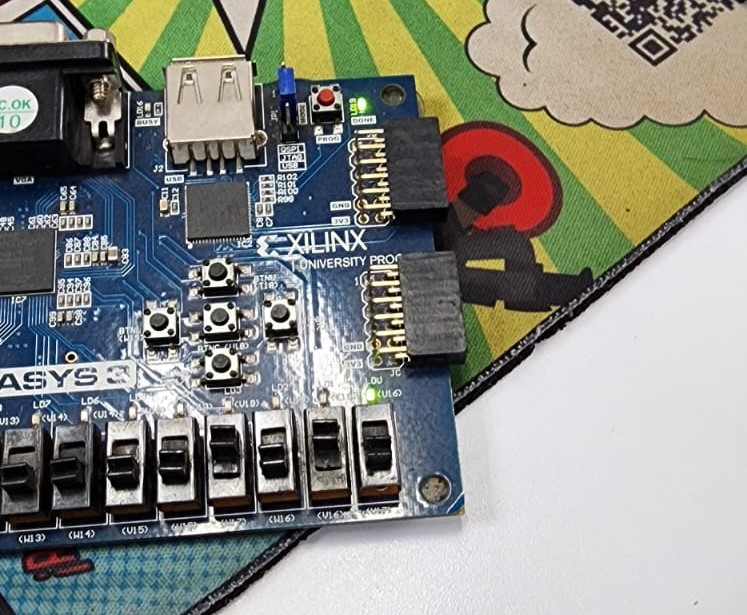
\includegraphics[width=0.8\linewidth]{images/diagrams/watertank/watertank5.jpg}
		\caption{Watertank element 5}
		\label{Watertank element 5 Apendix}
	\end{figure}

	\begin{figure}[H]
		\centering
		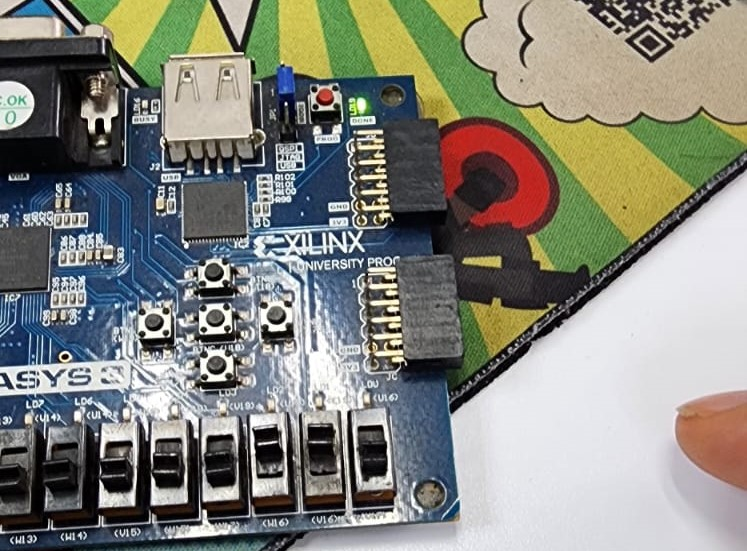
\includegraphics[width=0.8\linewidth]{images/diagrams/watertank/watertank6.jpg}
		\caption{Watertank element 6}
		\label{Watertank element 6 Apendix}
	\end{figure}

	\begin{figure}[H]
		\centering
		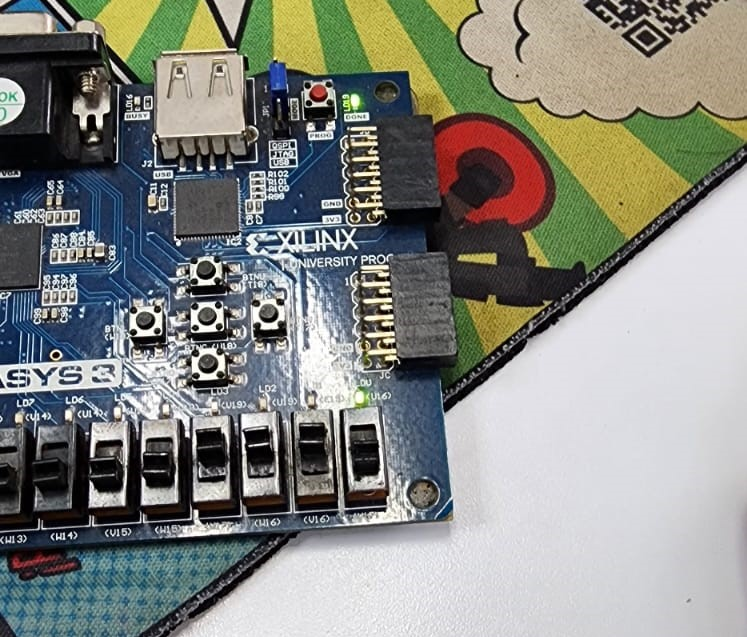
\includegraphics[width=0.8\linewidth]{images/diagrams/watertank/watertank7.jpg}
		\caption{Watertank element 7}
		\label{Watertank element 7 Apendix}
	\end{figure}

	\begin{figure}[H]
		\centering
		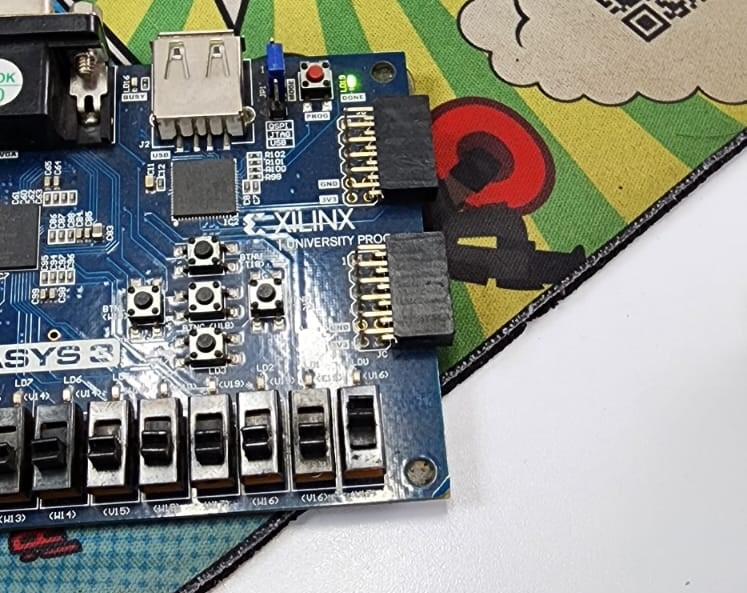
\includegraphics[width=1\linewidth]{images/diagrams/watertank/watertank8.jpg}
		\caption{Watertank element 8}
		\label{Watertank element 8 Apendix}
	\end{figure}

	\begin{figure}[H]
		\centering
		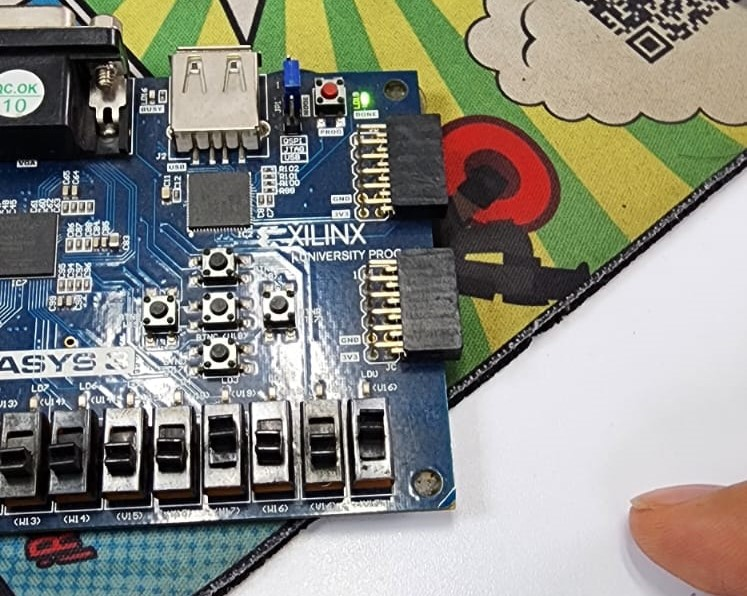
\includegraphics[width=1\linewidth]{images/diagrams/watertank/watertank9.jpg}
		\caption{Watertank element 9}
		\label{Watertank element 9 Apendix}
	\end{figure}

	\begin{figure}[H]
		\centering
		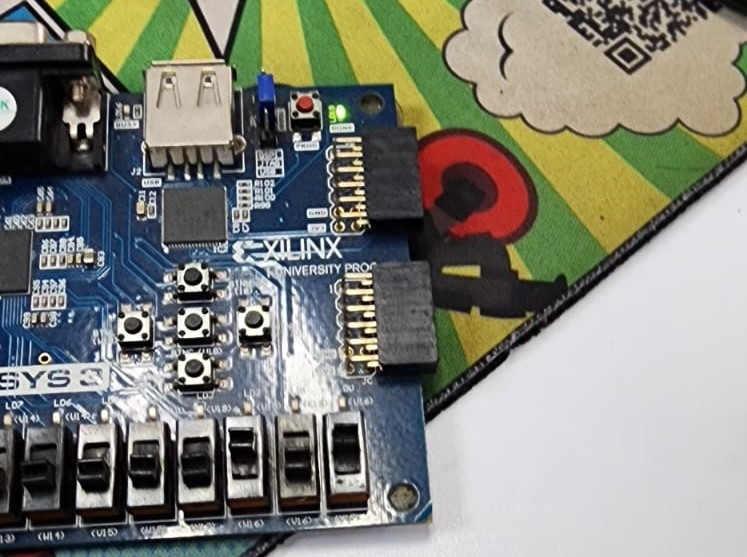
\includegraphics[width=1\linewidth]{images/diagrams/watertank/watertank10.jpg}
		\caption{Watertank element 10}
		\label{Watertank element 10 Apendix}
	\end{figure}

	\begin{figure}[H]
		\centering
		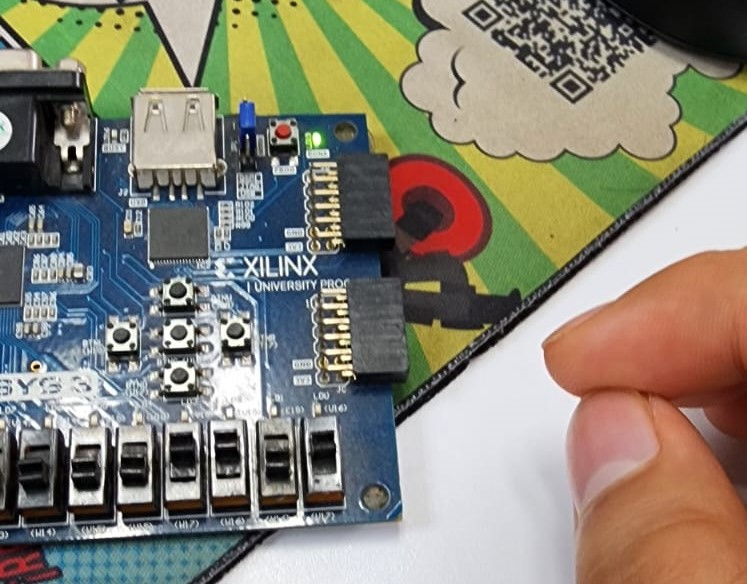
\includegraphics[width=1\linewidth]{images/diagrams/watertank/watertank11.jpg}
		\caption{Watertank element 11}
		\label{Watertank element 11 Apendix}
	\end{figure}

	\begin{figure}[H]
		\centering
		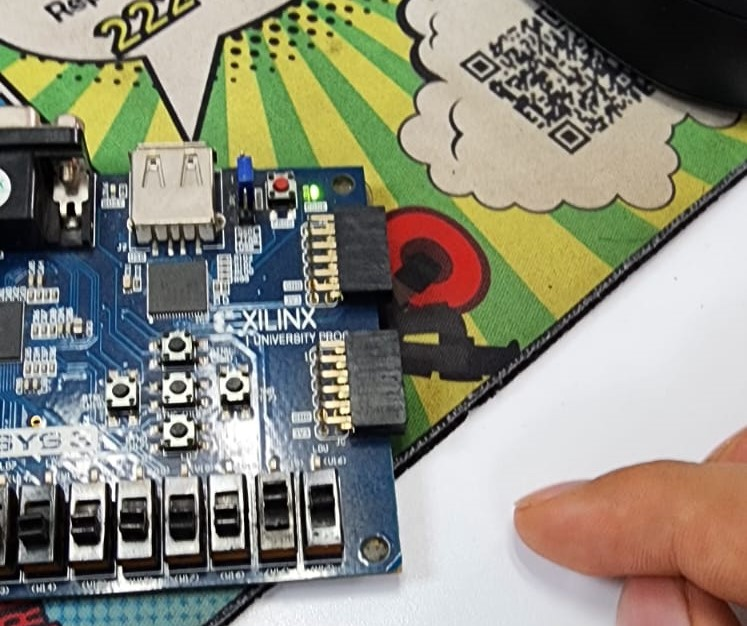
\includegraphics[width=1\linewidth]{images/diagrams/watertank/watertank12.jpg}
		\caption{Watertank element 12}
		\label{Watertank element 12 Apendix}
	\end{figure}

	\begin{figure}[H]
		\centering
		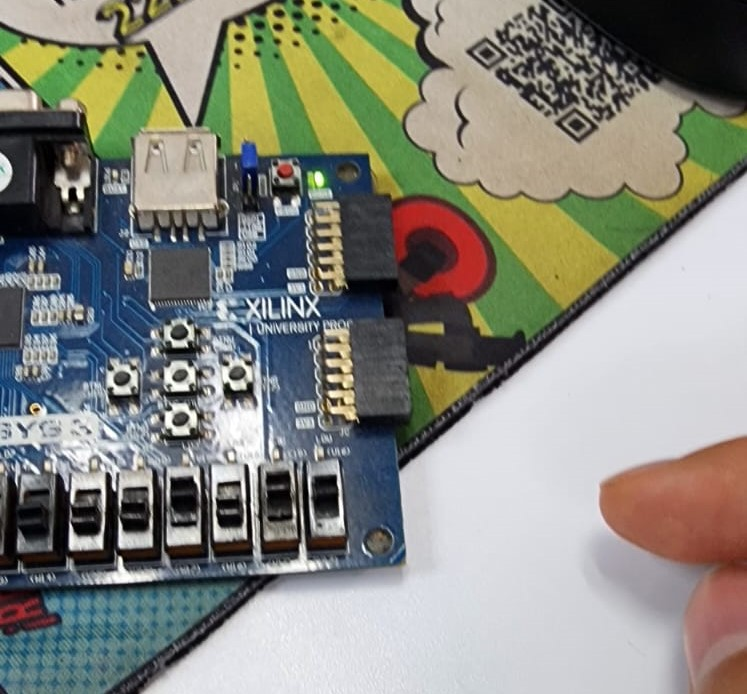
\includegraphics[width=1\linewidth]{images/diagrams/watertank/watertank13.jpg}
		\caption{Watertank element 13}
		\label{Watertank element 13 Apendix}
	\end{figure}

	\begin{figure}[H]
		\centering
		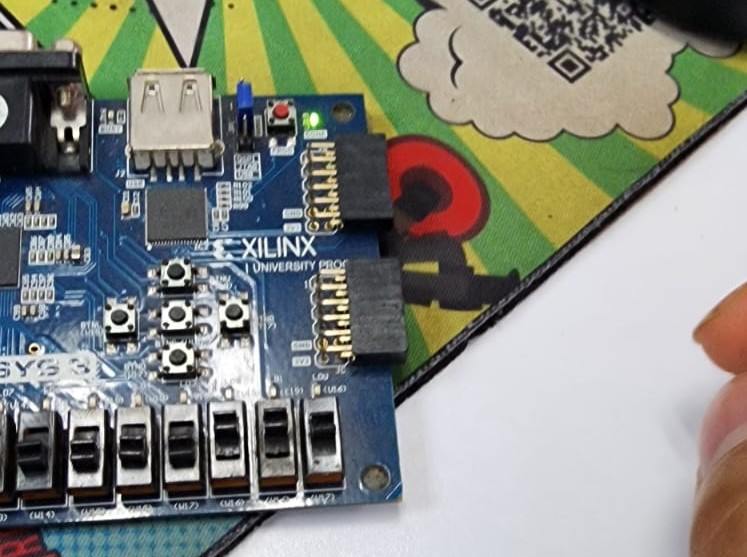
\includegraphics[width=1\linewidth]{images/diagrams/watertank/watertank14.jpg}
		\caption{Watertank element 14}
		\label{Watertank element 14 Apendix}
	\end{figure}

	\begin{figure}[H]
		\centering
		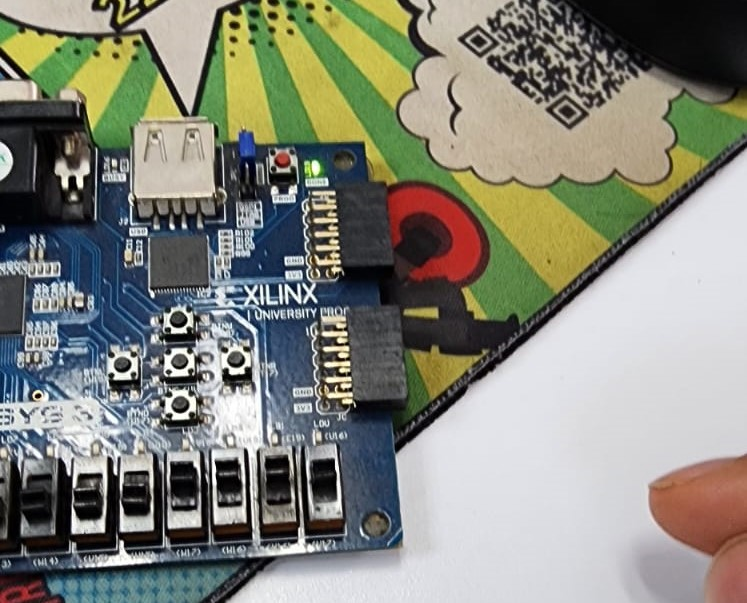
\includegraphics[width=1\linewidth]{images/diagrams/watertank/watertank15.jpg}
		\caption{Watertank element 15}
		\label{Watertank element 15 Apendix}
	\end{figure}

	\begin{figure}[H]
		\centering
		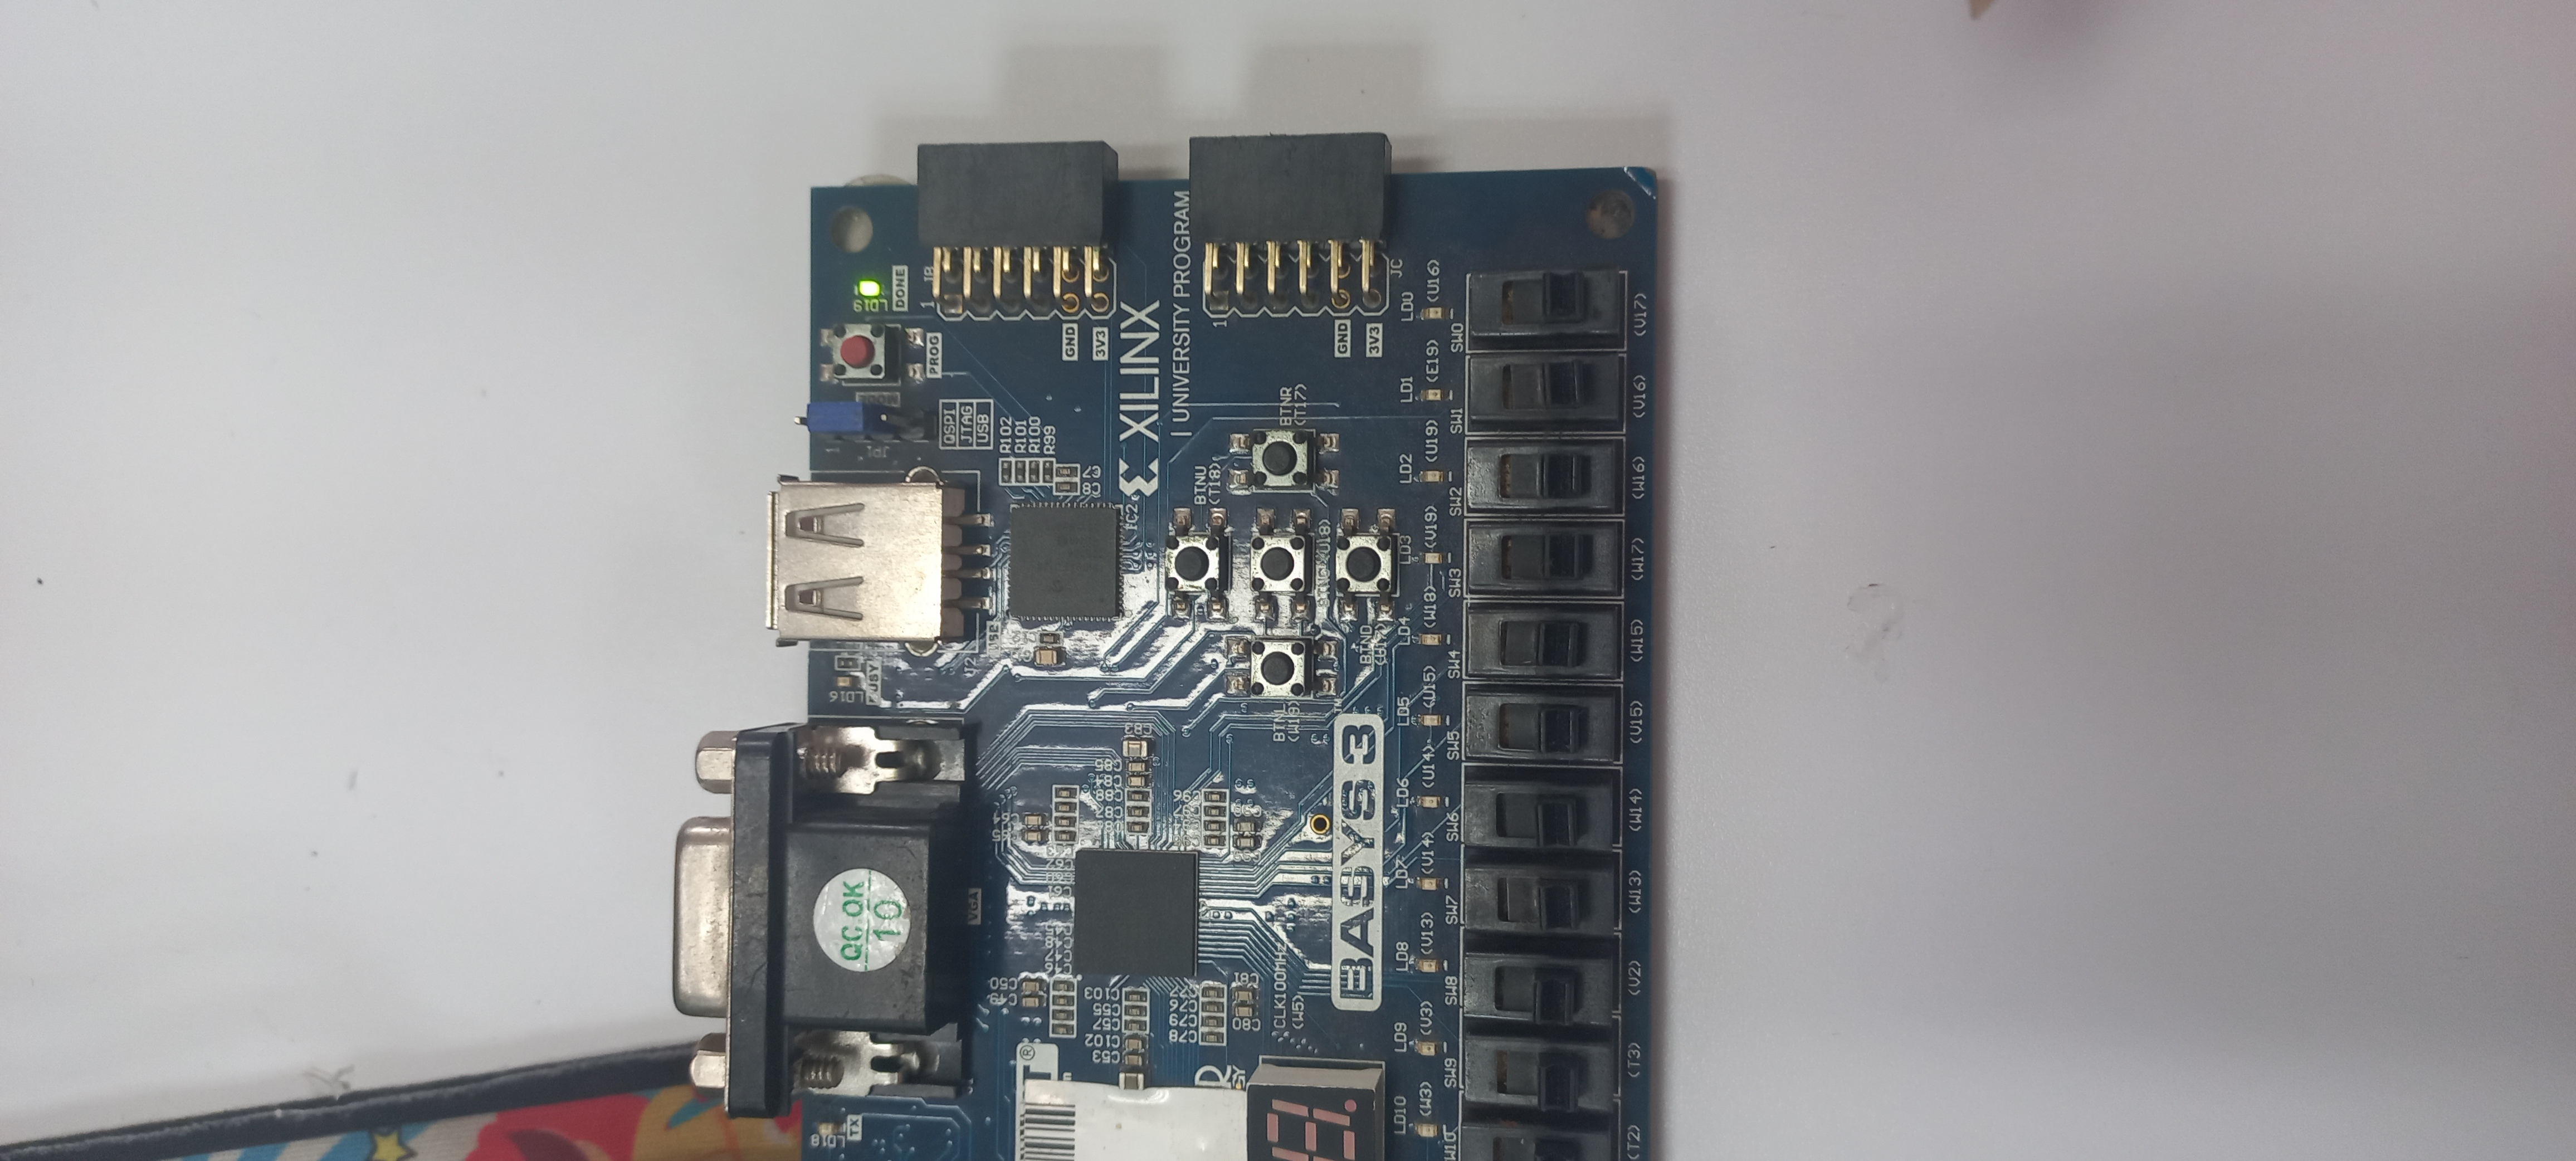
\includegraphics[width=1\linewidth]{images/diagrams/coin-selector/coin-selector0.jpg}
		\caption{Coin selector element 0}
		\label{Coin selector element 0 Apendix}
	\end{figure}

	\begin{figure}[H]
		\centering
		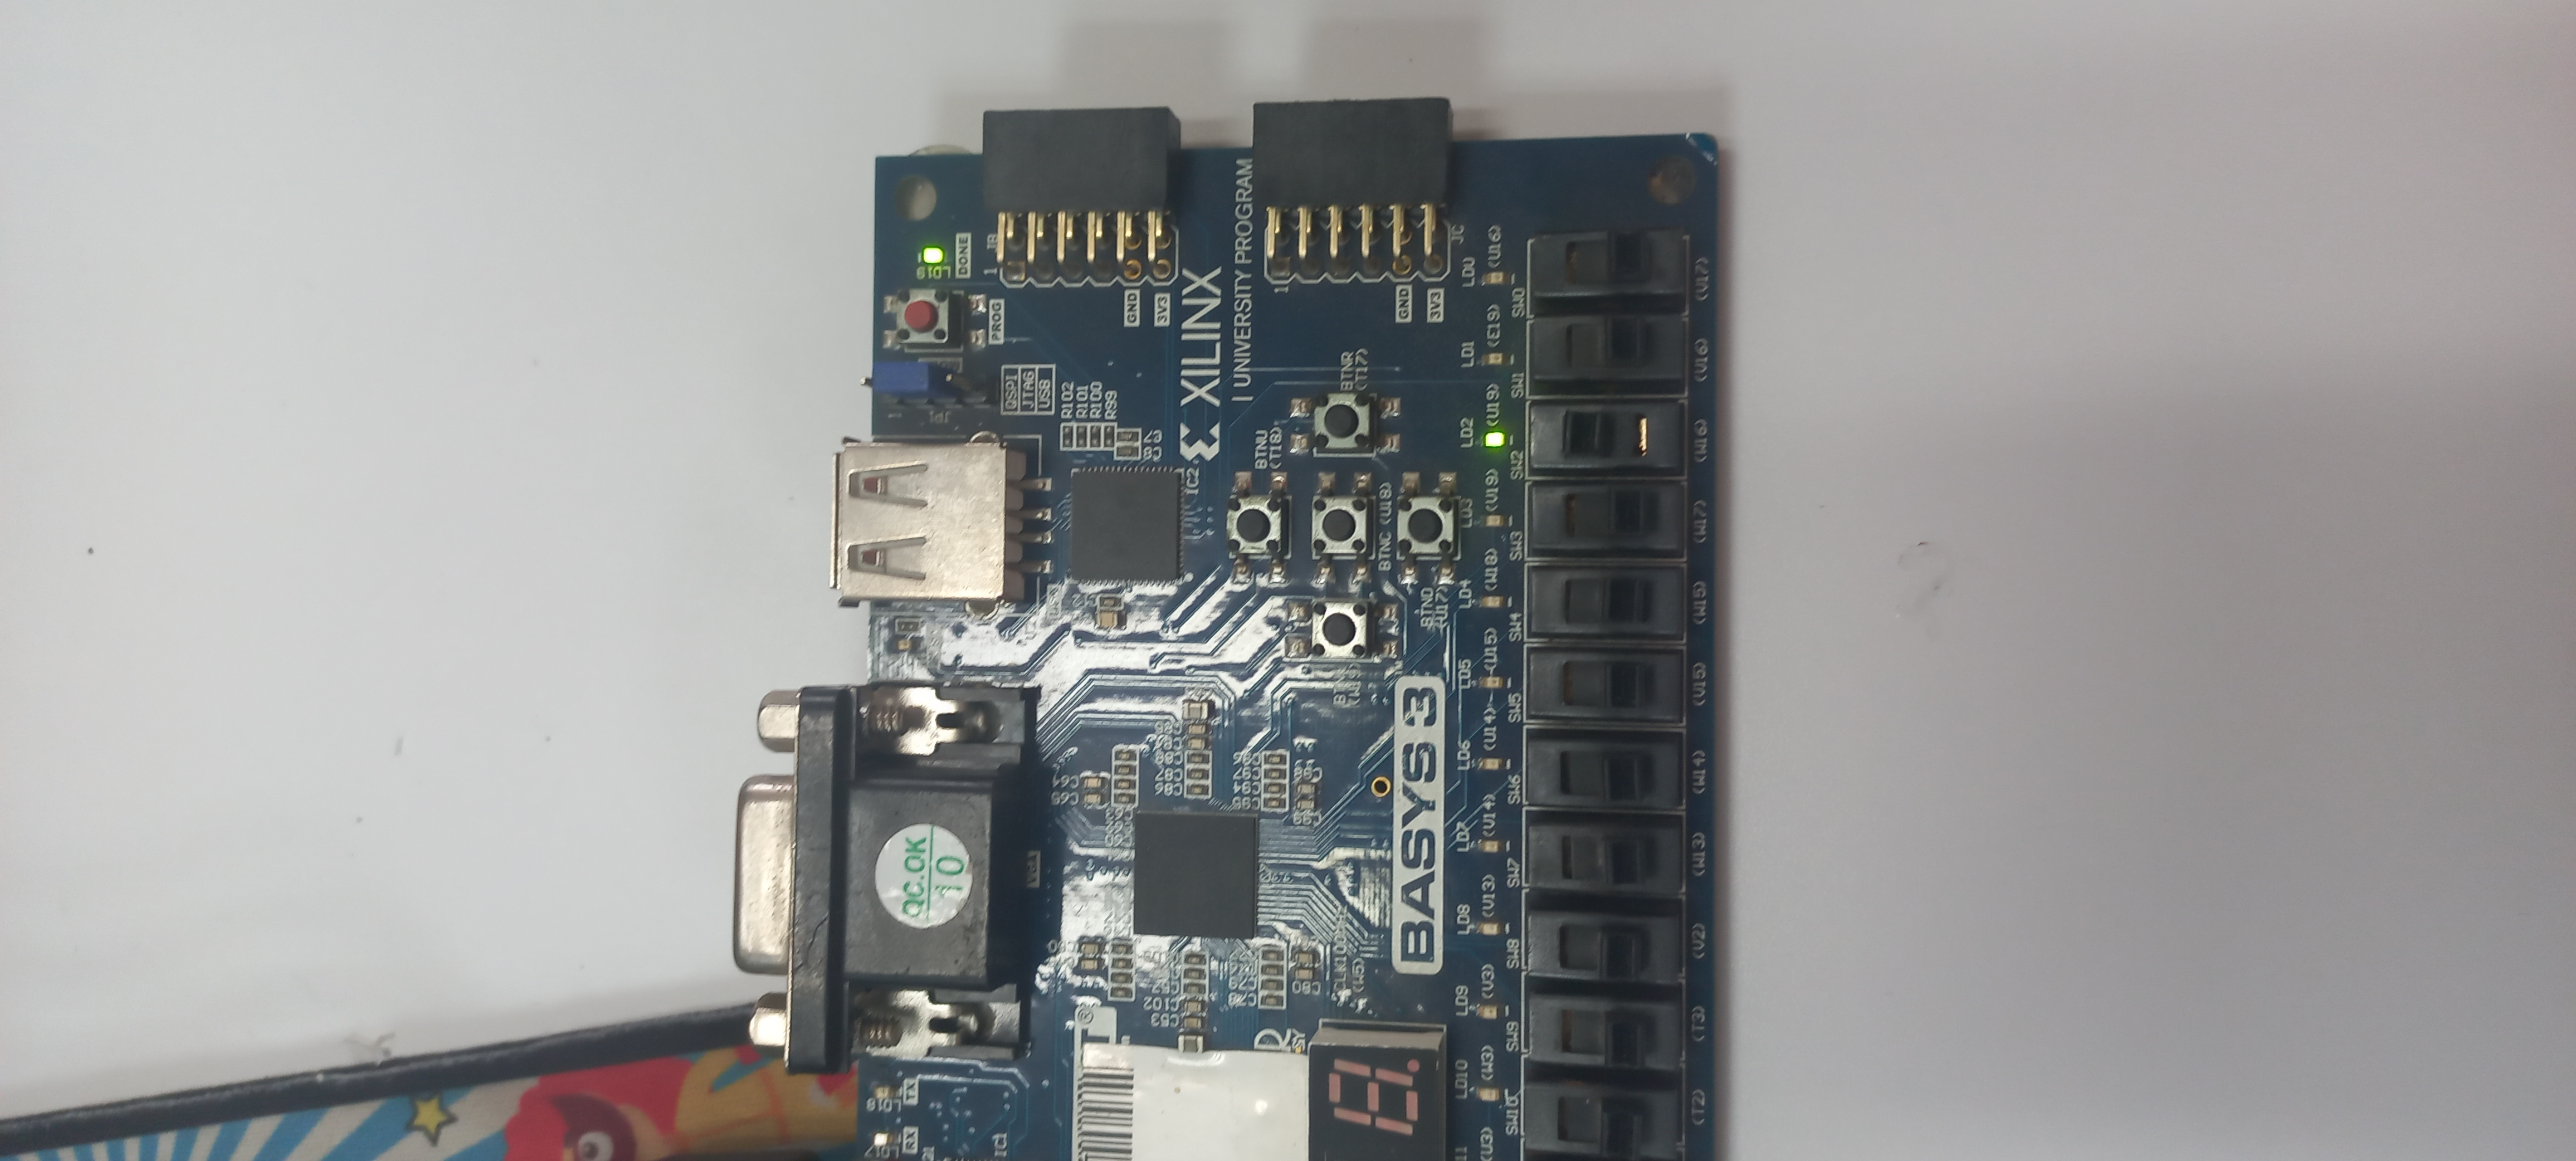
\includegraphics[width=1\linewidth]{images/diagrams/coin-selector/coin-selector1.jpg}
		\caption{Coin selector element 1}
		\label{Coin selector element 1 Apendix}
	\end{figure}

	\begin{figure}[H]
		\centering
		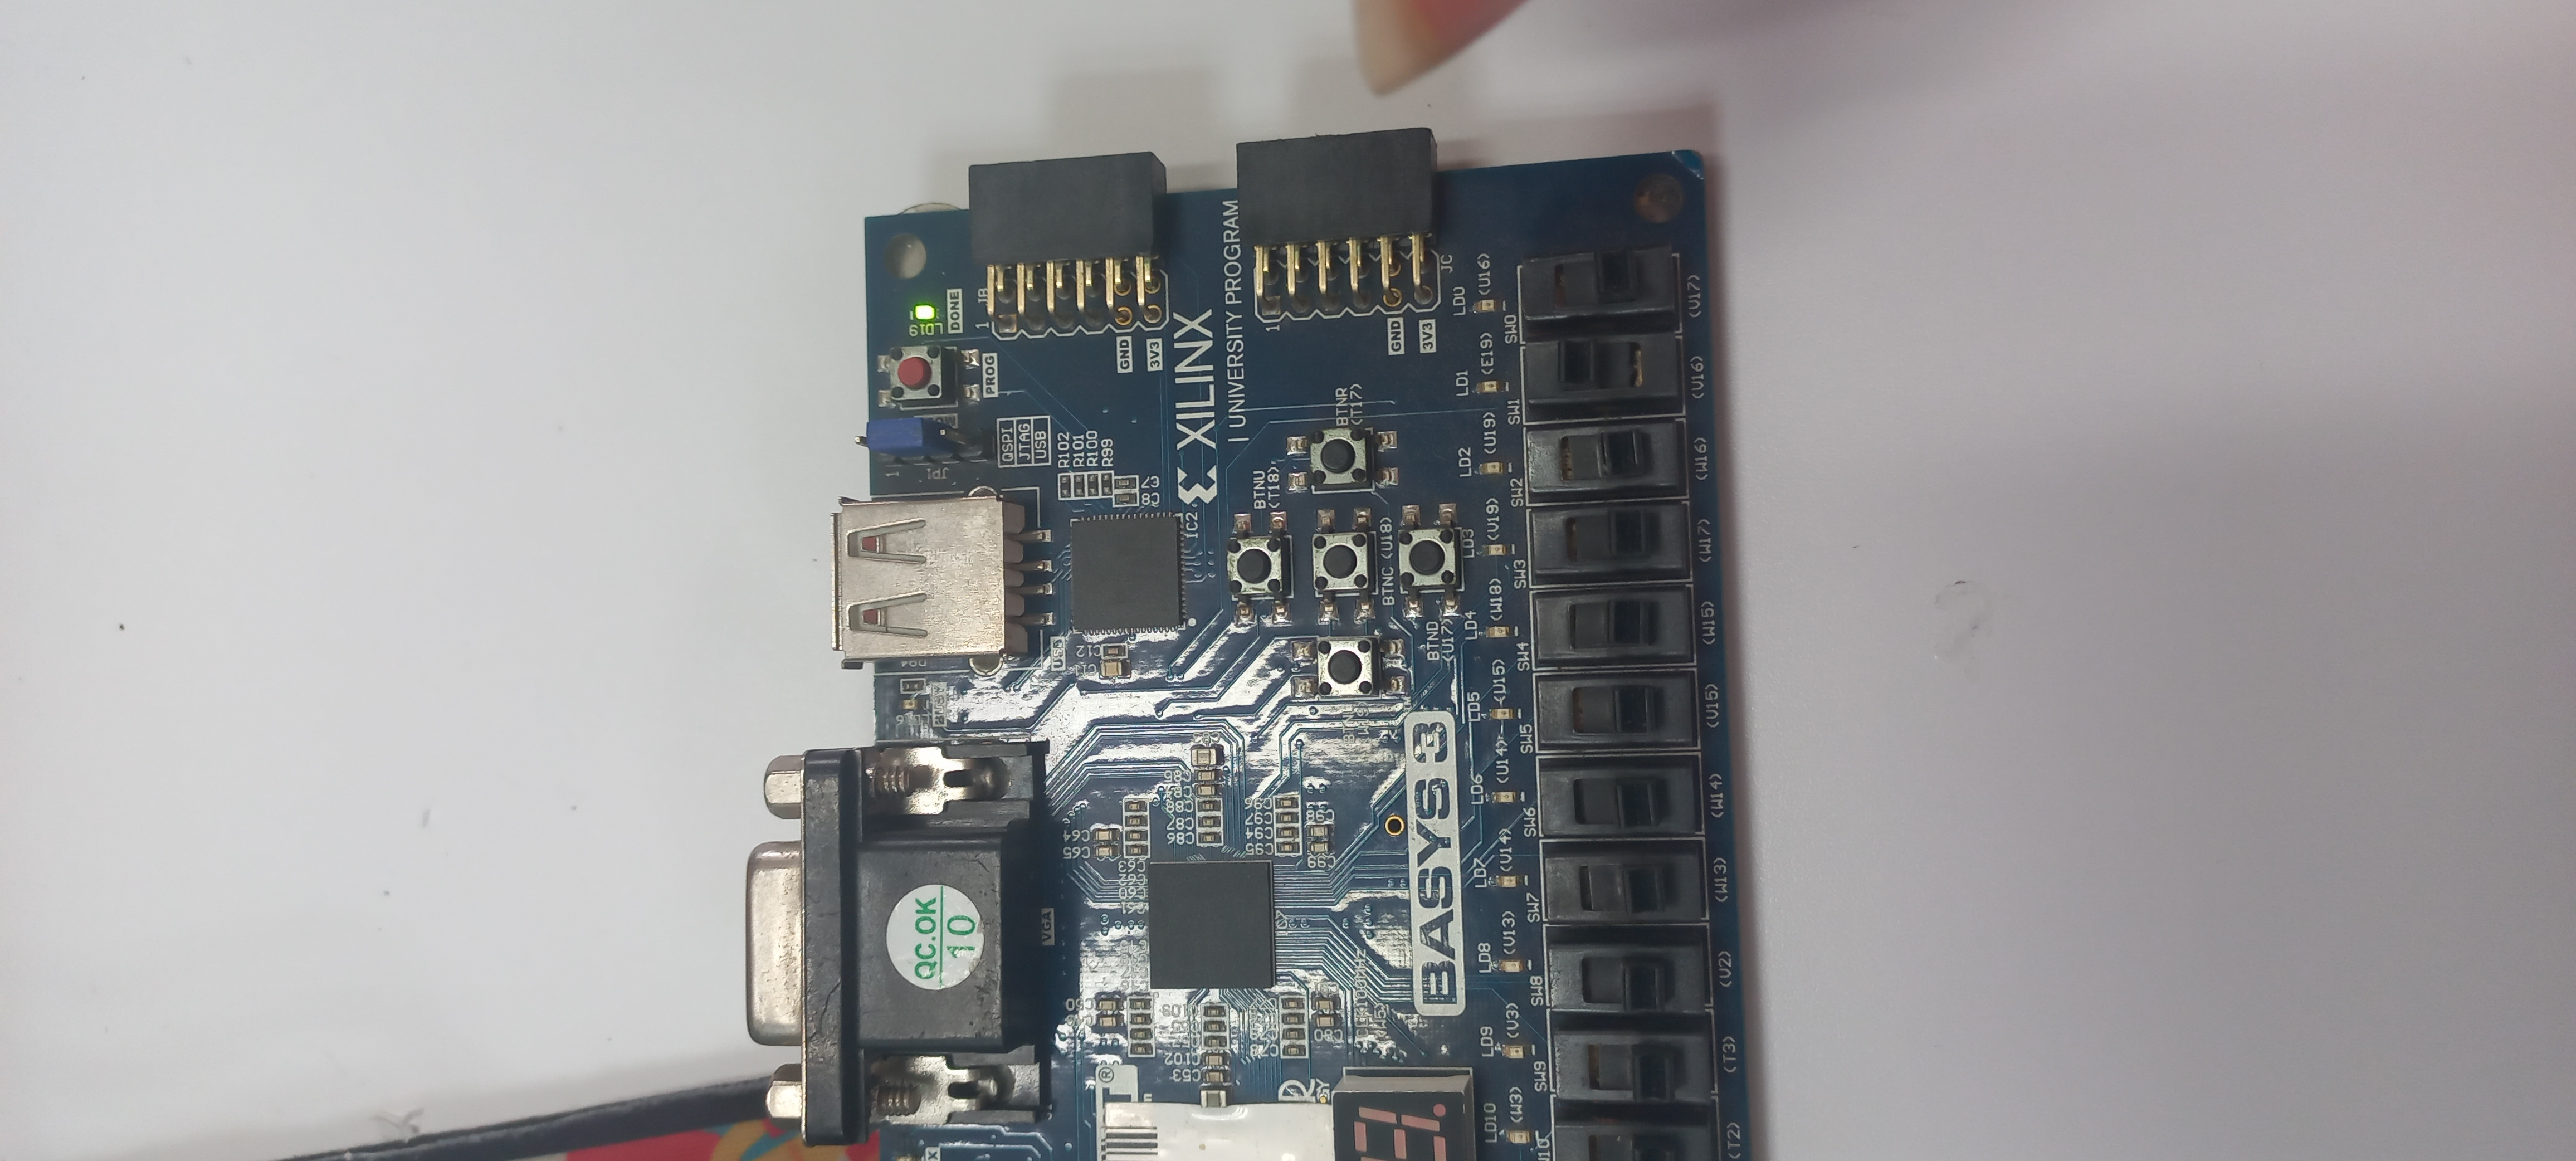
\includegraphics[width=1\linewidth]{images/diagrams/coin-selector/coin-selector2.jpg}
		\caption{Coin selector element 2}
		\label{Coin selector element 2 Apendix}
	\end{figure}

	\begin{figure}[H]
		\centering
		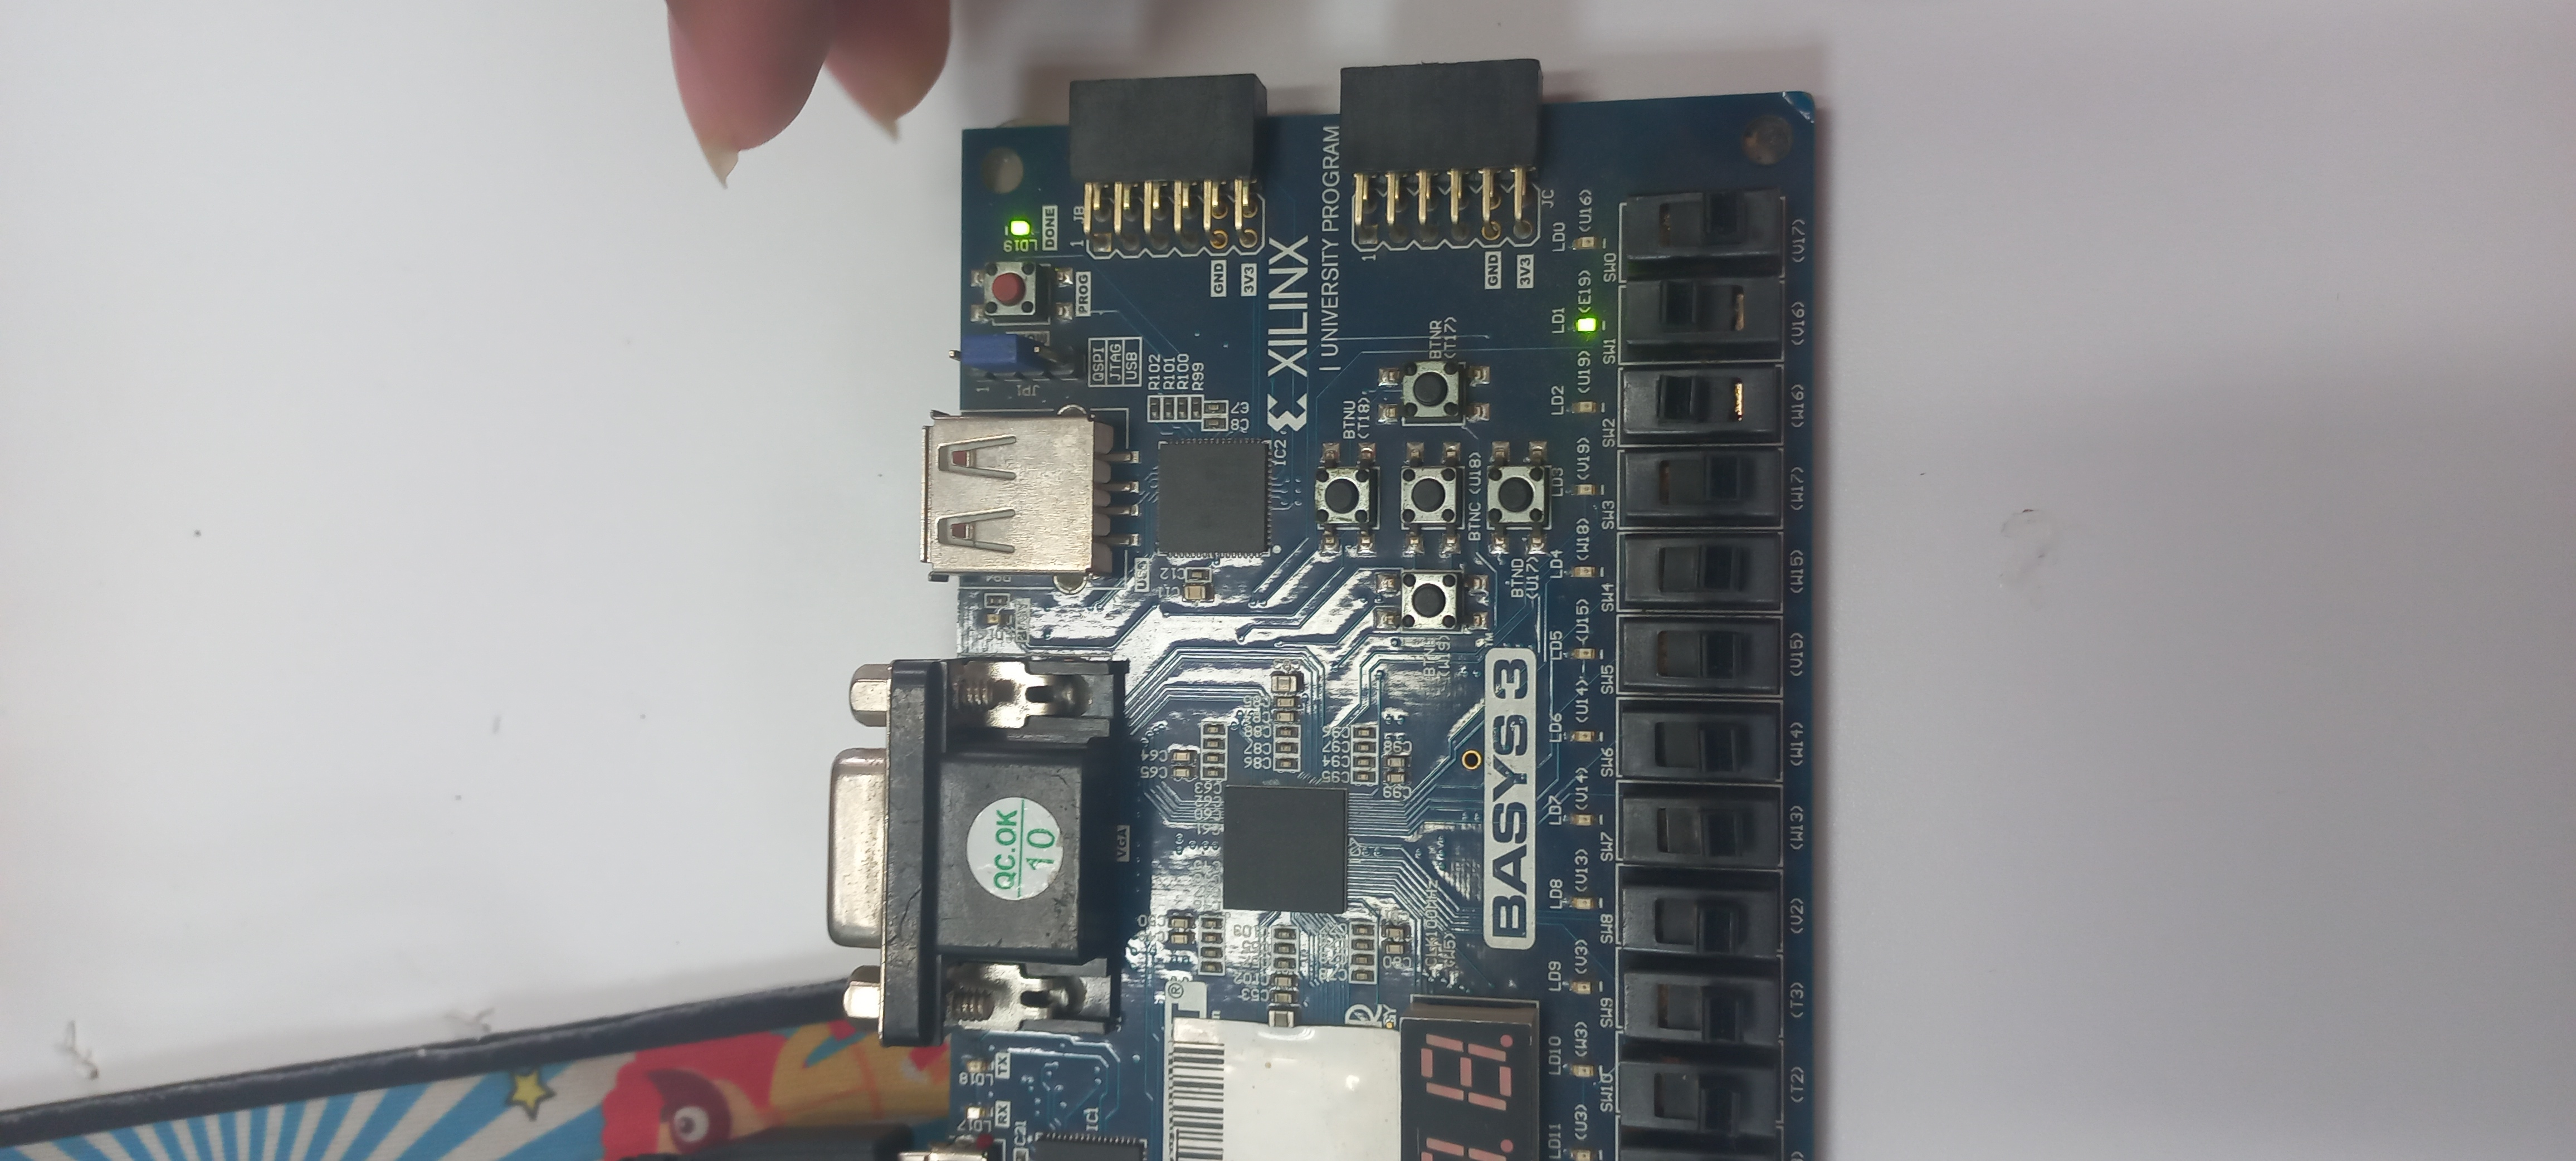
\includegraphics[width=1\linewidth]{images/diagrams/coin-selector/coin-selector3.jpg}
		\caption{Coin selector element 3}
		\label{Coin selector element 3 Apendix}
	\end{figure}

	\begin{figure}[H]
		\centering
		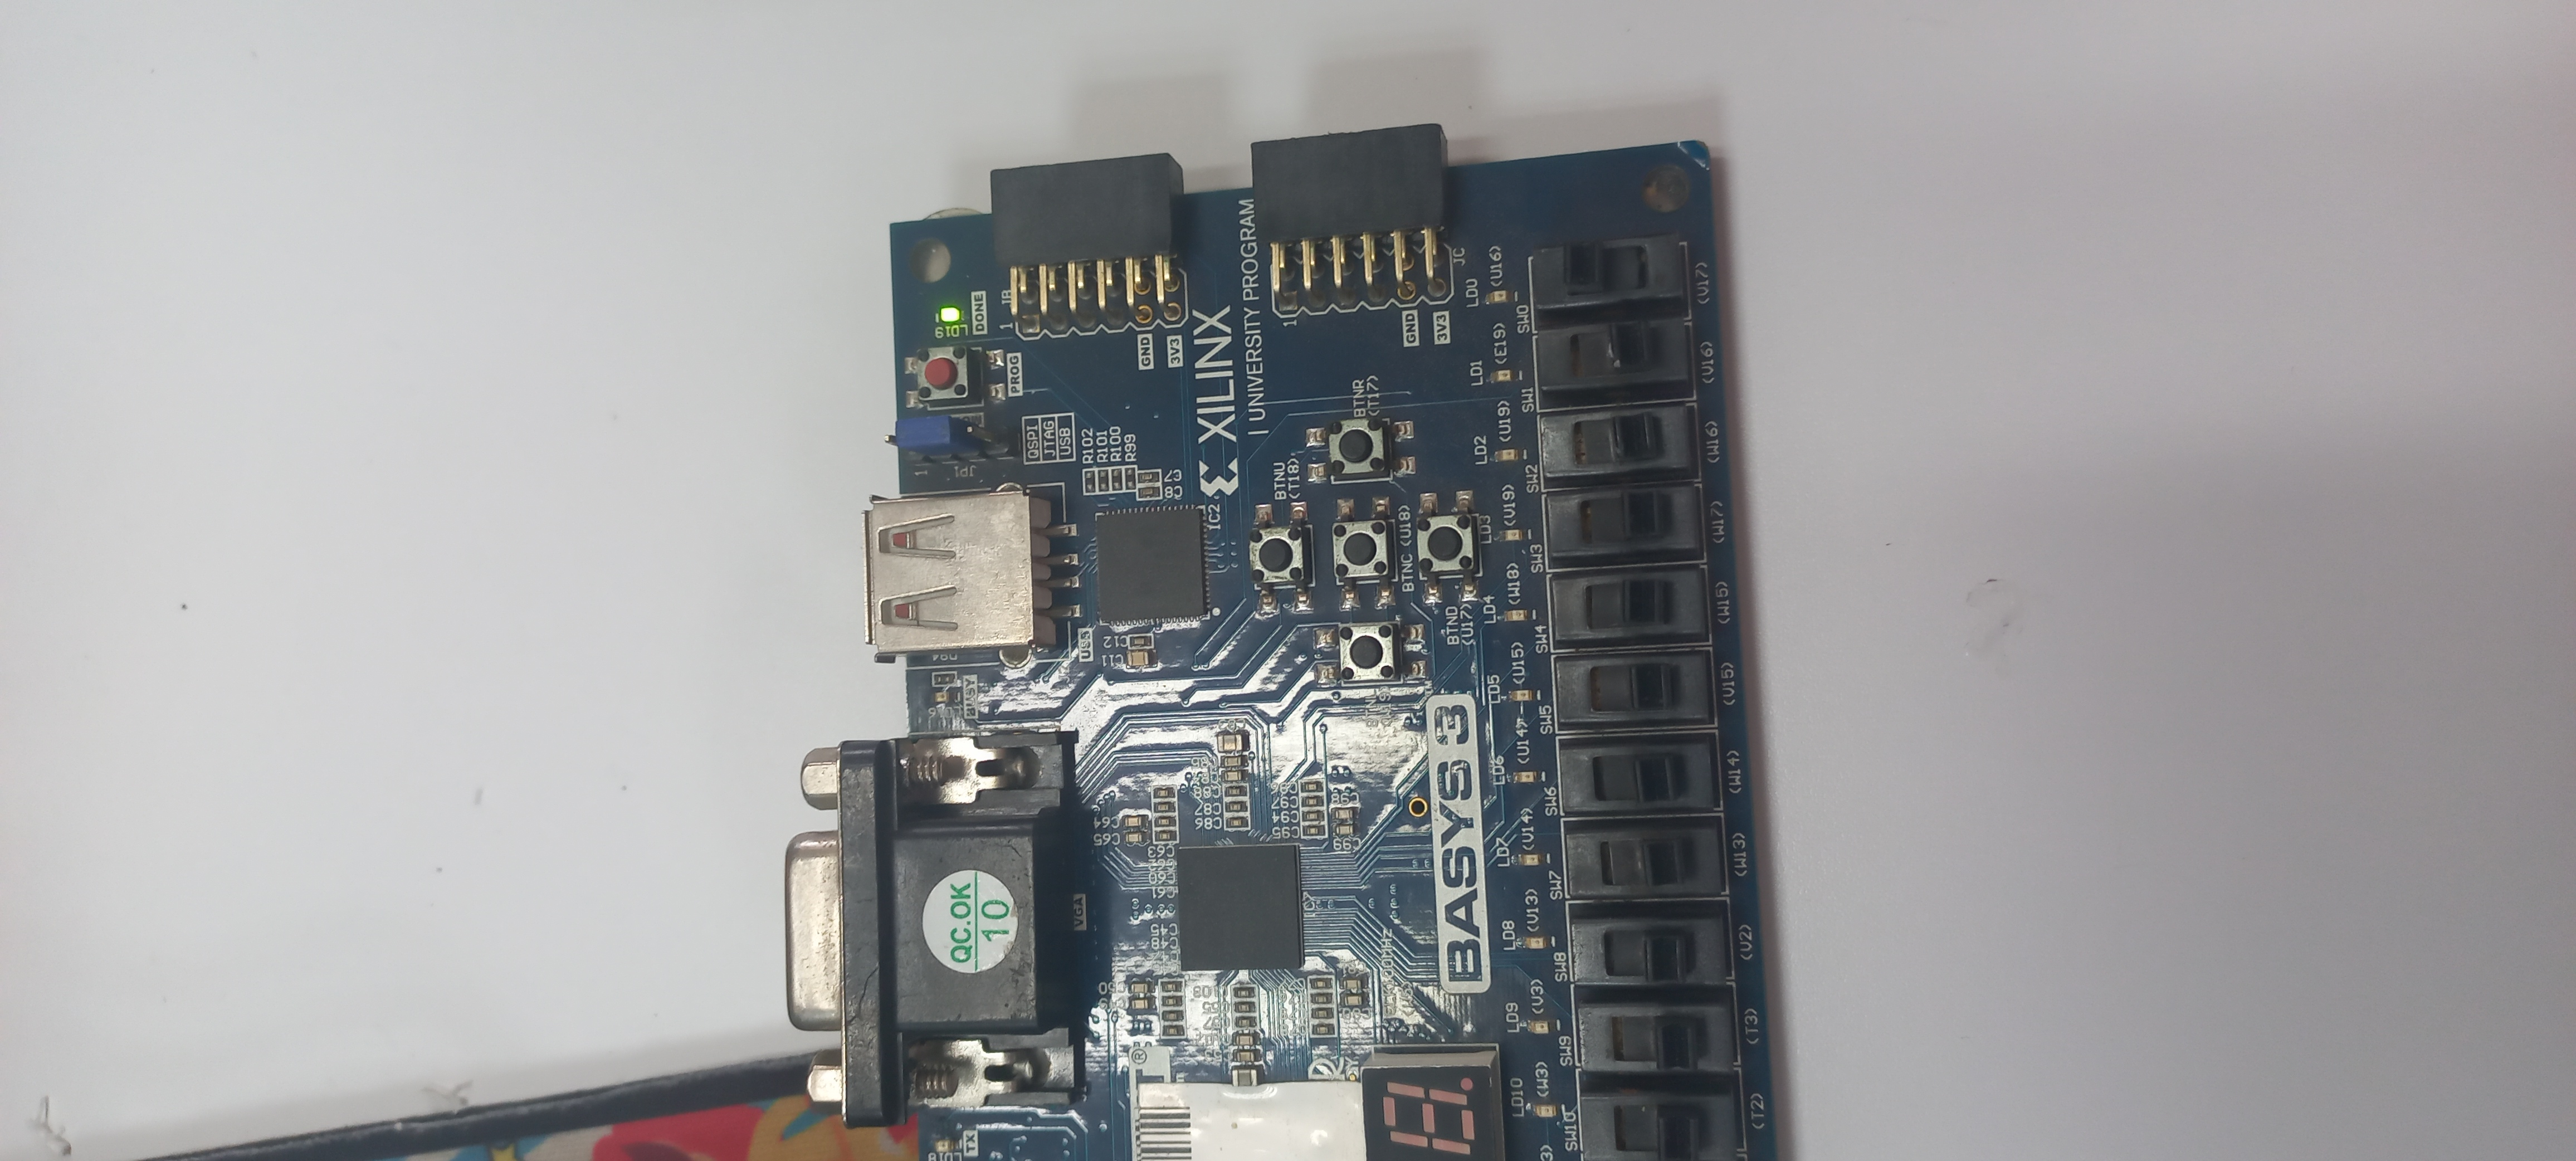
\includegraphics[width=1\linewidth]{images/diagrams/coin-selector/coin-selector4.jpg}
		\caption{Coin selector element 4}
		\label{Coin selector element 4 Apendix}
	\end{figure}

	\begin{figure}[H]
		\centering
		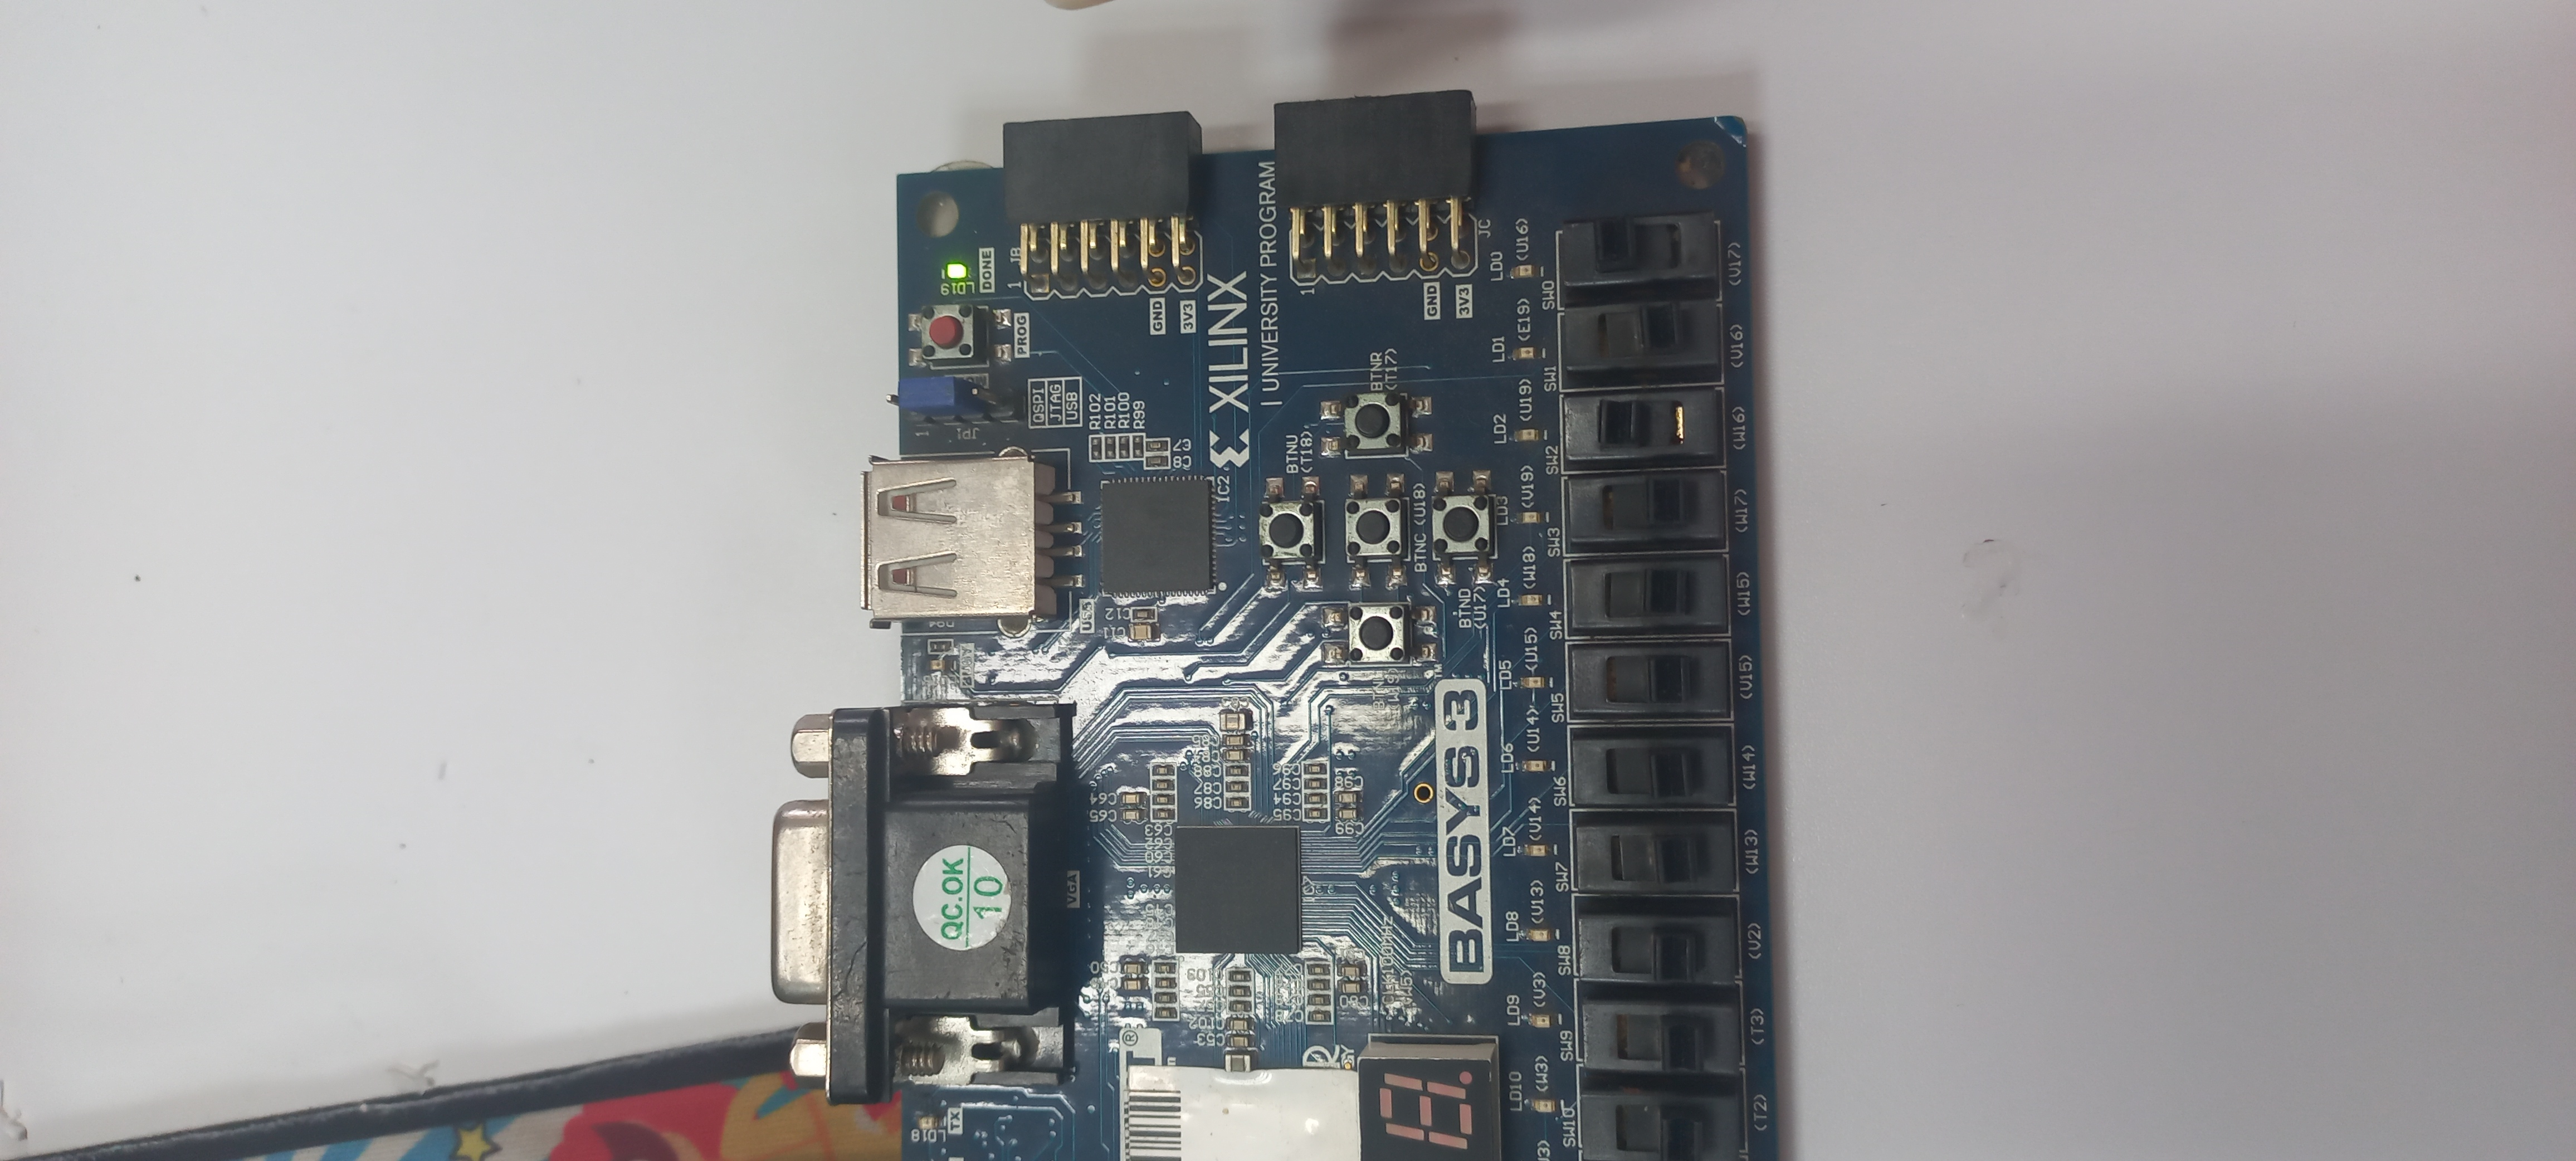
\includegraphics[width=1\linewidth]{images/diagrams/coin-selector/coin-selector5.jpg}
		\caption{Coin selector element 5}
		\label{Coin selector element 5 Apendix}
	\end{figure}

	\begin{figure}[H]
		\centering
		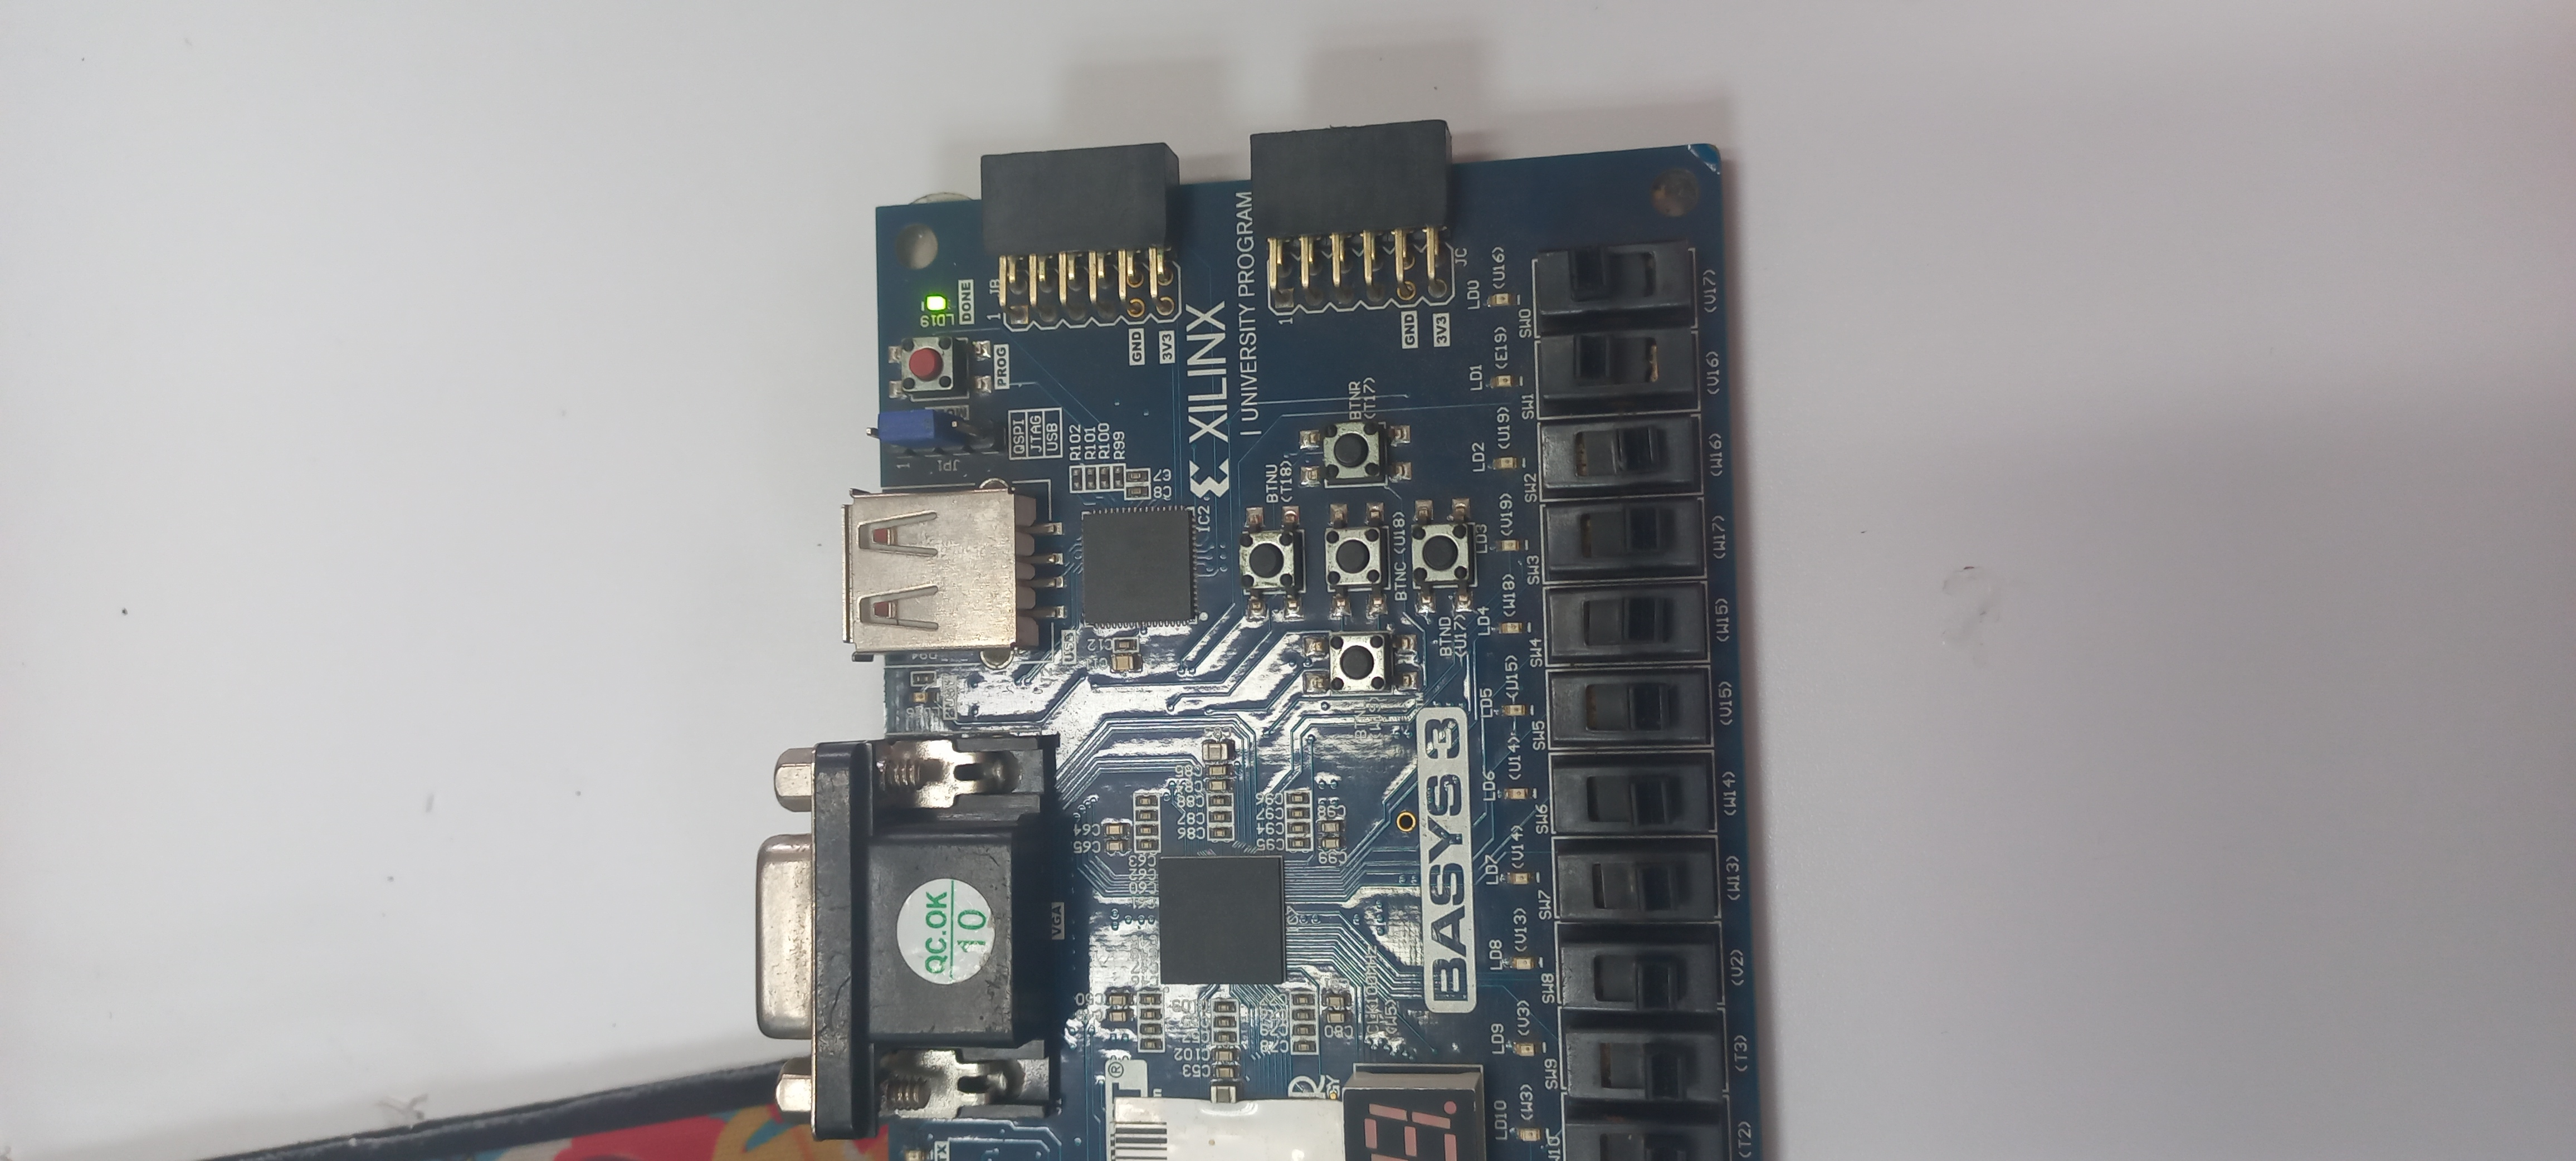
\includegraphics[width=0.8\linewidth]{images/diagrams/coin-selector/coin-selector6.jpg}
		\caption{Coin selector element 6}
		\label{Coin selector element 6 Apendix}
	\end{figure}

	\begin{figure}[H]
		\centering
		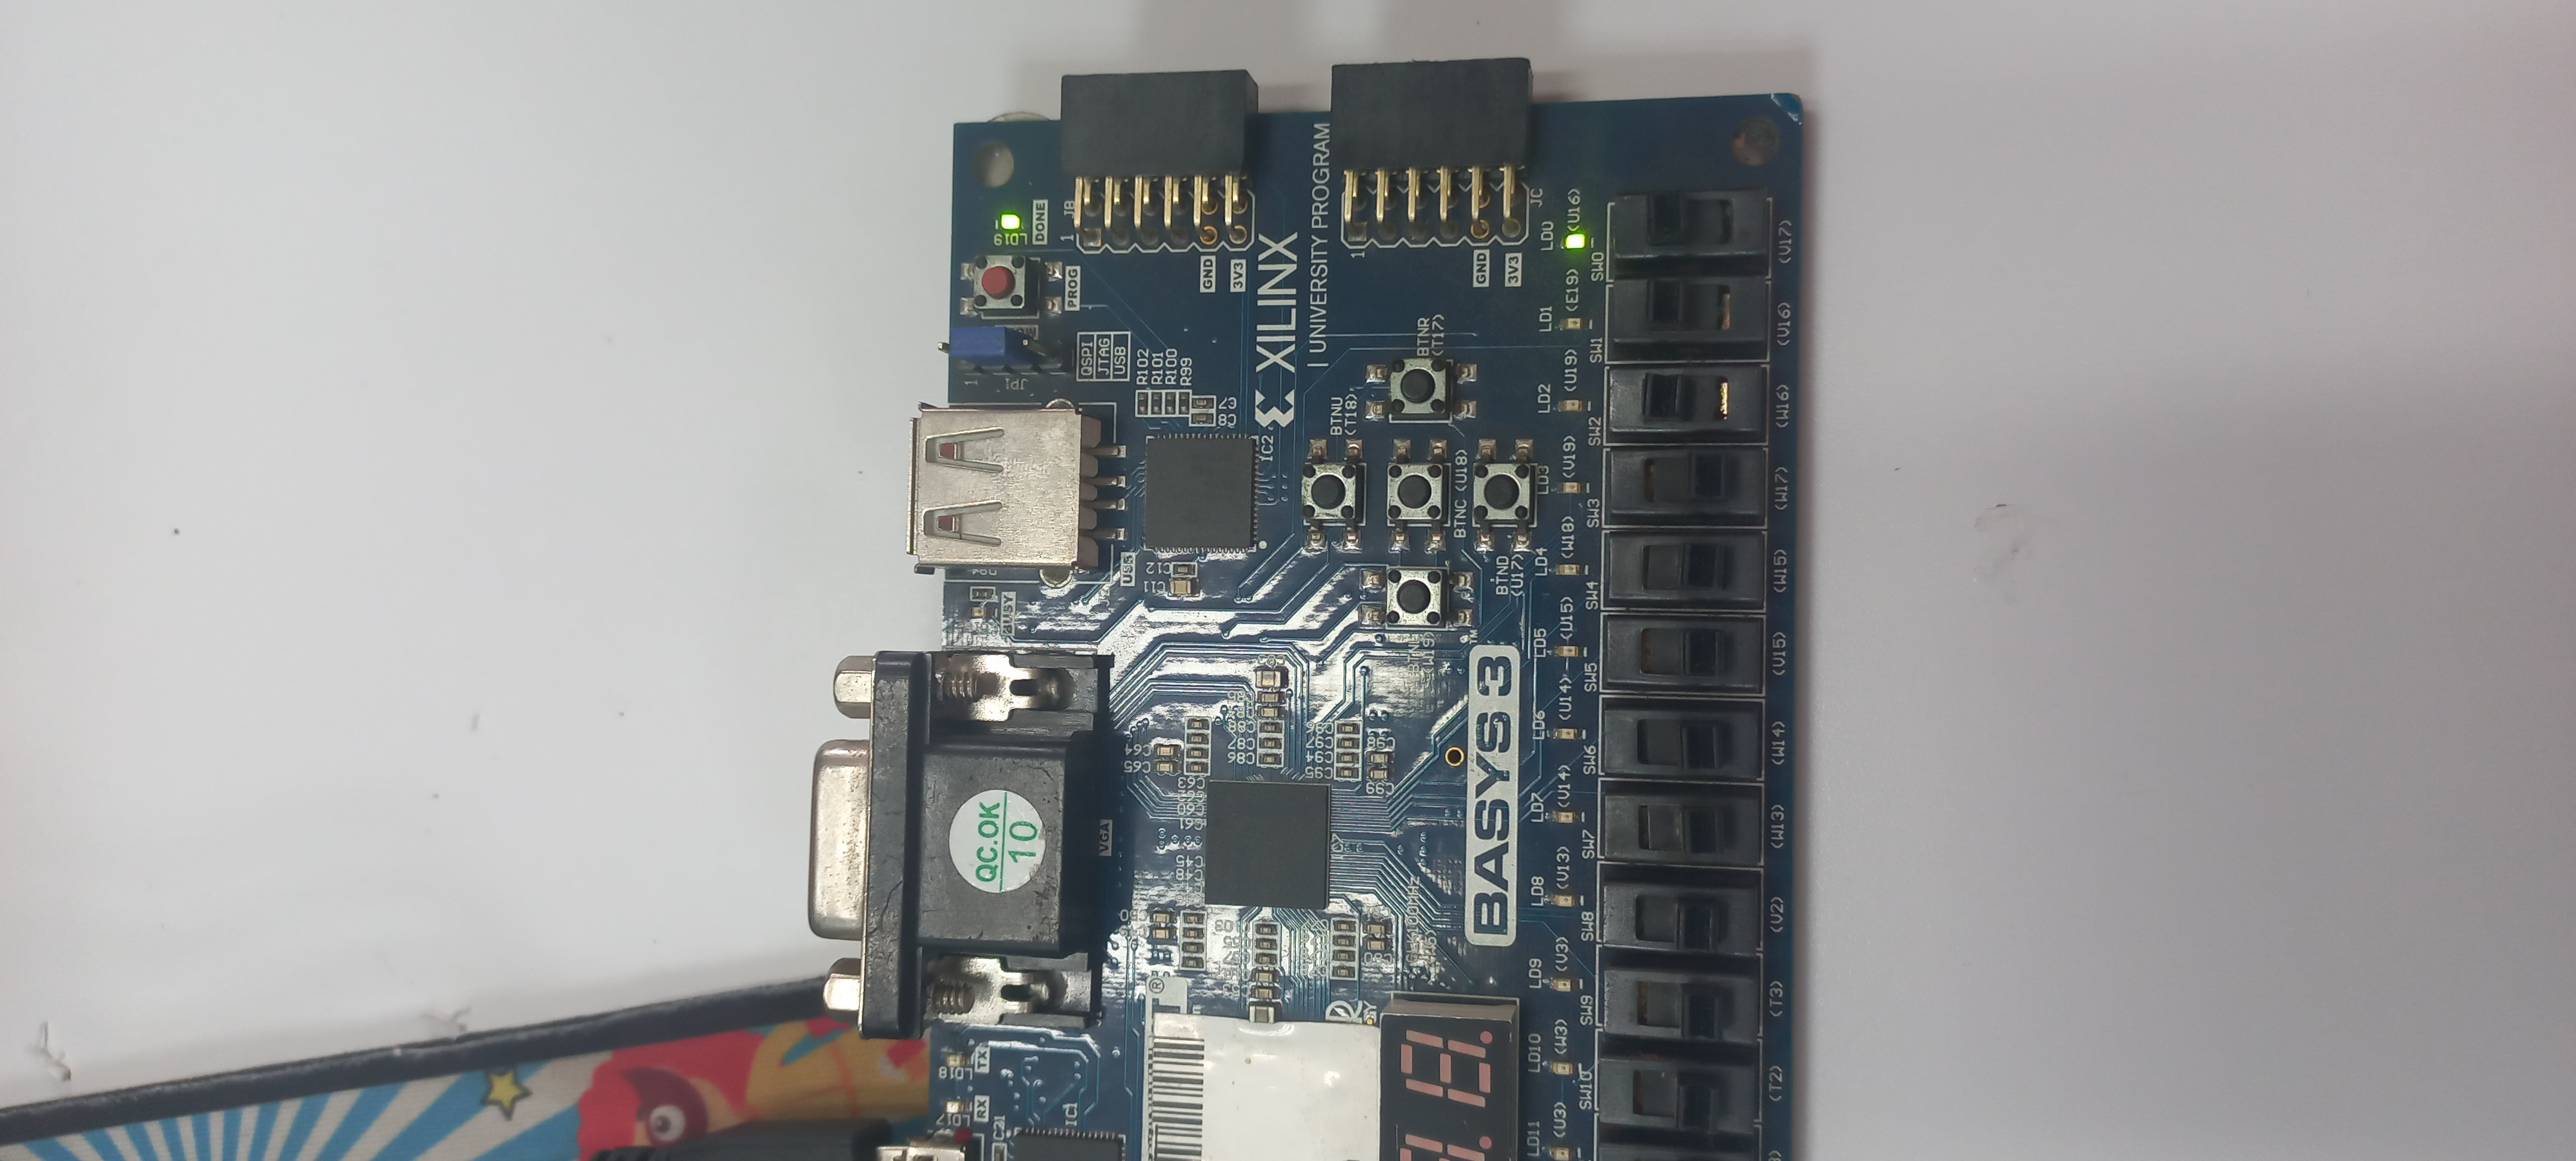
\includegraphics[width=0.8\linewidth]{images/diagrams/coin-selector/coin-selector7.jpg}
		\caption{Coin selector element 7}
		\label{Coin selector element 7 Apendix}
	\end{figure}

	\section{Karnaugh maps and tables}\label{Karnaugh maps and tables}

	\begin{figure}[H]
		\centering
		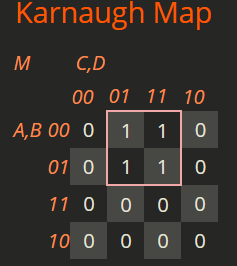
\includegraphics[width=0.6\linewidth]{images/k-maps/watertank.png}
		\caption{Watertank Karnaugh map}
		\label{Watertank Karnaugh map solution Apendix}
	\end{figure}

	\begin{table}[H]
		\centering
		\caption{Watertank truth table}
		\vspace*{1em}
		\begin{tabular}{|l|l|l|l|l|}
			\hline
			A & B & C & D & M \\ \hline
			0 & 0 & 0 & 0 & 0 \\ \hline
			0 & 0 & 0 & 1 & 1 \\ \hline
			0 & 0 & 1 & 0 & 0 \\ \hline
			0 & 0 & 1 & 1 & 1 \\ \hline
			0 & 1 & 0 & 0 & 0 \\ \hline
			0 & 1 & 0 & 1 & 1 \\ \hline
			0 & 1 & 1 & 0 & 0 \\ \hline
			0 & 1 & 1 & 1 & 1 \\ \hline
			1 & 0 & 0 & 0 & 0 \\ \hline
			1 & 0 & 0 & 1 & 0 \\ \hline
			1 & 0 & 1 & 0 & 0 \\ \hline
			1 & 0 & 1 & 1 & 0 \\ \hline
			1 & 1 & 0 & 0 & 0 \\ \hline
			1 & 1 & 0 & 1 & 0 \\ \hline
			1 & 1 & 1 & 0 & 0 \\ \hline
			1 & 1 & 1 & 1 & 0 \\ \hline
		\end{tabular}
	\end{table}


	\begin{table}[H]
		\centering
		\caption{Coin selector truth table}
		\vspace*{1em}
		\begin{tabular}{|l|l|l|l|l|l|}
			\hline
			A & B & C & Diez & Cinco & Uno \\ \hline
			0 & 0 & 0 & 0    & 0     & 0   \\ \hline
			0 & 0 & 1 & 0    & 0     & 1   \\ \hline
			0 & 1 & 0 & 0    & 0     & 0   \\ \hline
			0 & 1 & 1 & 0    & 1     & 0   \\ \hline
			1 & 0 & 0 & 0    & 0     & 0   \\ \hline
			1 & 0 & 1 & 0    & 0     & 0   \\ \hline
			1 & 1 & 0 & 0    & 0     & 0   \\ \hline
			1 & 1 & 1 & 1    & 0     & 0   \\ \hline
		\end{tabular}
	\end{table}

	\bibliographystyle{bst/IEEEtran}
	\bibliography{bib/bibliografia}
\end{multicols}
\end{document}